% !TEX root = ../document.tex

\chapter{ADS-B 系统简介}

\section{ADS-B 系统的技术原理}

\subsection{概述}

ADS-B(Automatic Dependent Surveillance-Broadcast,广播式自动相关监视)技术是现代空中交通管理中一项非常重要的监视手段,该项监视技术无需地面设备询问,它以自动广播的方式,按照固定的频率向其它航空器或者地面空中交通管制中心广播飞机的状态信息,这些信息是通过一定的渠道从飞机本身或者卫星设备上获取的,通常这些信息由飞机呼号、位置、高度、速度和航向等信息组成。ADS-B 的信息以报文形式传输,通过空-空、空-地数据链广播式传播。

\begin{figure}[htbp]
\centering
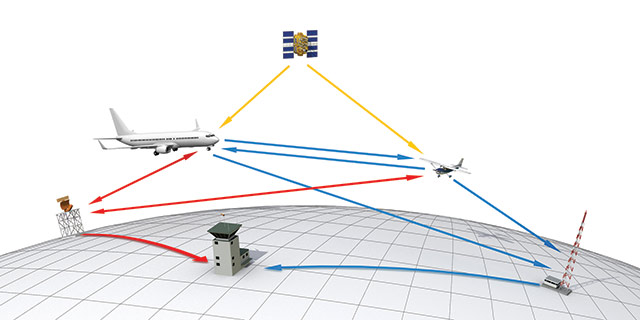
\includegraphics[width=13cm]{pic/Advocacy_ADS_B.jpg}
\caption{ADS-B 系统工作原理}
\label{fig:Advocacy_ADS_B}
\end{figure}

ADS-B 分为两个部分:ADS-B In 和 ADS-B Out。ADS-B In 是系统的接收部分,负责接收 ADS-B 信息;ADS-B Out 是安装有发射器的面板,负责向其他飞机和地面站发送信号,这将告诉其他飞机和地面站本飞行器的位置、速度和航向等信息。注意 ADS-B Out 设备是始终安装在飞机上的并且需要经过认证,这个设备不可拆卸。这样做的目的是为了防止在未授权的情况下,人为关闭 ADS-B 等其他监视跟踪设备,致使无法追踪飞机位置,导致像马来西亚航空 MH370 航班那样的事故。

\subsection{数据链类型}

为了避免频率过载,ADS-B 可以使用不同的数据链以使用不同的频率收/发数据。目前可以支持 ADS-B 技术的数据链主要有三种,分别是基于 S 模式的 1090ES、978UAT(Universal Access Transceiver,通用访问收发机)数据链和 VDL Mode4(VHFDigital Link,模式 4 甚高频数据链)。这三种数据链技术各有优缺点,当前美国同时使用 1090ES 和 UAT 数据链,欧洲同时使用 1090ES 和 VDL Mode4 数据链,而澳大利亚仅使用 1090ES 数据链。目前只有 S 模式 1090ES 数据链获得国际无线电组织的批准,同时国际民航组织对 1090ES 数据链的支持力度最大,标准也最完善。你可以拥有多种 ADS-B 产品:仅 978 In、978 In\&Out、仅 1090ES Out 等等。

\subsubsection{1090ES 数据链}

1090ES 是一个使用扩展震荡信标(Extended Squitter)的改进的 S 模式转发器(使用转发器的 1090MHz 频率),
使用高度要超过 18000 英尺。

\subsubsection{978UAT 数据链}

在美国,18000 英尺以下的高度层使用这种数据链,它在 978MHz 上传输,在技术上称为通用访问收发机(UAT)。

\subsubsection{VDL Mode4 数据链}

\section{ADS-B 系统的应用意义}

当前世界范围内空中交通流量与密度不断增加,在未来的几十年内,随着无人机的普及,有人驾驶飞机和无人机都需要在同一片空域正常且无冲突地运行。下一代空中交通管理系统是处理空中流量爆发式增长和保证数十亿乘客安全的关键所在。ADS-B 是这一关键的核心技术,它的出现,将大幅提升航行监视系统的态势感知能力。当前我国民航空中监视系统的中流砥柱是二次雷达,这种基于传统通信模式的的监视设备一般可以报告飞机的身份识别代码、高度代码、飞机地址等信息,由于消息长度限制,不能提供位置完整性报告。为了保持空中交通的效率,同时保证安全,需要提供更精确的监测系统和消息的完整性,ADS-B 可以克服当前雷达系统的局限性并提高其监视性能,增加空域容量,在无法部署雷达的内陆地区,ADS-B 能为飞机提供优于雷达间隔标准的虚拟雷达管制服务;在有雷达覆盖地区,在不增加雷达设备的情况下,能够以较低代价辅助现有雷达系统。ADS-B 系统并非一个独立的监视系统,它对外部系统的高度依赖,比如 GPS 系统将为其提供位置报告,正因为此,ADS-B 的监视精度可以提高至 10 米量级,监视数据更新速度可达 1 秒 1 次。另外,ADS-B 技术成本较低,其地面站建设成本是传统二次雷达的九分之一。ADS-B 技术将为传统空管监视领域带来重大变革。

\section{ADS-B 系统的发展现状}

国际民航组织于第十一届航行大会确定 ADS-B 技术为全球新航行技术的主要发展方向,目前全球各国都在不懈推广 ADS-B 技术的应用。

\renewcommand\arraystretch{1.5}
\begin{table}[htbp]
\centering
\caption{Countries with ADS-B Out mandates and proposals}
\label{tab:Countries_with_ADS-B_Out_mandates_and_proposals}
\begin{tabular}[b]{|p{2cm}<{\raggedleft}|p{13cm}<{\raggedright}|}
\hline
\textbf{美国} & The FAA has mandated ADS-B Out capabilities for flight after January 1, 2020, for flight in most airspace where a Mode C transponder is required today. There is one significant exception: ADS-B also will be required in certain airspace above the Gulf of Mexico. At this time, only the United States is allowing the 978UAT datalink for ADS-B Out. If you plan to fly in ADS-B airspace outside of the United States, a 1090ES datalink—using a Mode S Extended Squitter transponder—will be required.
\par
美国联邦航空局已要求在 2020 年 1 月 1 日之后飞行的 ADS-B Out 飞行能力,用于今天需要模式 C 转发器的大部分空域。有一个重要的例外:在墨西哥湾以上的某个空域也需要 ADS-B。目前,只有美国允许将 978UAT 数据链路用于 ADS-B 输出。如果您计划在美国以外的 ADS-B 空域飞行,则需要使用模式 S 扩展 Squitter 转发器的 1090ES 数据链路。\\
\hline
\textbf{澳大利亚} & 1090ES required for all IFR operations. Foreign-registered aircraft equipped with transponders are exempted below FL290 until June 6, 2020.
\par
所有 IFR 操作都需要 1090ES。 配备转发器的外国注册飞机在 2020 年 6 月 6 日之前免于低于 FL290  \\
\hline
\textbf{加拿大} & Currently no mandate, but operators who voluntarily equip with 1090ES (particularly in the Hudson Bay and nearby oceanic airspace) can receive a higher level of service. Nav Canada is part of a joint air traffic surveillance venture, Aireon, installing ADS-B equipment on low-earth-orbit satellites. Nav Canada will be the launch customer when the service becomes available in 2018, and initially intends to incorporate 1090ES ADS-B into North Atlantic airspace.
\par
目前没有授权,但自愿装备 1090ES(特别是在哈德逊湾和附近的海洋空域)的运营商可以获得更高水平的服务。Nav Canada 是 Aireon 联合空中交通监控机构的一部分,在低地球轨道卫星上安装 ADS-B 设备。Nav Canada 将在 2018 年提供服务时成为发射客户,并且最初打算将 1090ES ADS-B 纳入北大西洋空域。\\
\hline
\textbf{欧洲} & 1090ES required for IFR aircraft with a MTOW exceeding 12,566 pounds or maximum cruise airspeed faster than 250 KTAS. Mandatory for new-production aircraft, and must be retrofitted into all aircraft by June 7, 2020. (Dates have slipped from original timetable.)
\par
IFR 飞机所需的 1090ES,MTOW 超过 12,566 磅,或最大巡航空速超过 250 KTAS。对于新生产的飞机必须使用,并且必须在 2020 年 6 月 7 日之前对所有飞机进行改装。(日期已经从原来的时间表中滑落。) \\
\hline
\textbf{香港} & 所有空域 FL290 及以上需要 1090ES \\
\hline
\textbf{印度尼西亚} & FL290 及以上需要 1090ES \\
\hline
\textbf{墨西哥} & 从 2020 年 1 月 1 日开始,在平均海平面 10000 英尺以上 A、B、C、E 级空域以及其他指定的空域需要 1090ES;目前要求在墨西哥湾的 E 级空域和墨西哥海岸 12 海里以内平均海平面 3000 英尺以上需要 1090ES \\
\hline
\textbf{新加坡} & 指定的航空公司需要 1090ES \\
\hline
\textbf{斯里兰卡} & Colombo 终端控制区(TMA,Colombo Terminal Control Area),FL290 及以上需要需要 1090ES \\
\hline
\textbf{台湾} & 所有空域 FL290 及以上需要 1090ES \\
\hline
\textbf{越南} & 指定的航空公司需要 1090ES \\
\hline
\end{tabular}
\end{table}

\subsection{国外应用现状}

目前欧美等航空发达国家已制定本国和本地区的 ADS-B 实施规划,建立相关的规章和标准,开展验证与应用。

\subsubsection{北美地区}

在国外,美国是最先开展 ADS-B 技术研究和应用的国家之一,是美国 NextGen 计划的基础之一,帮助飞行员和空中交通管制员创建一个更安全、更高效的国家空域系统(NAS)。美国的 ADS-B 应用路线是:先通用航空,后商用运输。目前,在通用航空方面,美国已经完全实现使用 ADS-B 技术来为自己的航空器提供监视服务。

2016 年 9 月,美国联邦航空局(FAA)开始提供 500 美元奖励,以帮助通用航空运营商支付 ADS-B 设备和安装费用,并鼓励他们现在就装备。

FAA 要求在 2020 年之前,所有在受控空域飞行的飞机都必须安装有 ADS-B OUT,而对 ADS-B In 的安装没有强制要求。

2016 年,FAA 与墨西哥的空中交通服务提供商 SENEAM 合作,使用合资建立的 ADS-B 地面站扩展在墨西哥湾上空的 ADS-B 监视覆盖水平。新的地面站有助于飞行器飞过美国和墨西哥之间的墨西哥湾。

墨西哥的其他地面站对于空中交通路线提供无缝监控覆盖,使海湾地区的容量从每小时 75 架增加到约 85 架。到 2035 年,这些地面站将为美国-墨西哥领空边界提供更多的海湾航班,从而为运营商节省 7000 万美元。增加容量可减少高峰期的延误,从而节省飞机运营成本和乘客时间。

FAA 正在开发 Interval Management,这是一套借助 ADS-B 的能力对航班进行排队和分配的应用软件。间隔管理的精确间距可以在拥挤的空域内实现更高效的飞行路径,并最大限度地提高空域和机场利用率。这些功能需要新的航空电子设备、地面自动化、决策支持系统和程序。FAA 也在探索 ADS-B 在越来越多的商用太空飞行器发射方面的能力。FAA 也在和运营商和其他的 ANSPs 合作,以评估向海洋空域的管制方提供 ADS-B 数据潜在利益。减少分离标准的替代方法包括使用 ADS-B 或使用增强版本 ADS-C。

\subsubsection{澳大利亚}

澳大利亚的 ADS-B 应用水平也达到了很高的程度,该国地广人稀,雷达监视系统建设部署比较薄弱,鉴于这种情况,澳大利亚开始投资部署 ADS-B 系统以配合为数不多的航管雷达设备。

\subsubsection{欧洲}

欧洲各国 ADS-B 应用水平也在大力推进,当前位于欧洲中部的 OpenSky 感知网络的 ADS-B 系统可以捕捉到欧洲大约 30\% 的商业航班,其监视能力相当可观。ADS-B 也是欧洲单一天空计划(SESAR)的基石,欧盟(欧洲共同体和欧控)是 SESAR 的创始人。

欧洲 ADS-B 实施计划要求从 2015 年起,质量大于 5700kg 或速度超过 250 节的新飞行器当在以仪表飞行规则(IFR)下飞行时要装备 ADS-B Out,已经运营的飞机从 2017 年底开始进行改装,在 2020 年 ADS-B 监视系统需要开始运作\upcite{h2}。

\subsection{国内应用现状}

在 ADS-B 技术的研发应用方面,中国民航紧跟国际发展动态,努力与世界接轨。当今 ADS-B 监视技术已在中国民航处于实用阶段,截至 2014 年底,中国民航全行业运输飞机注册架数已达 2370 架,部分已完成 1090ES(1090Mhz Extended Squitter,1090 兆赫扩展断续脉冲)ADS-B OUT 机载设备加改装。中国民航在西部高原地区实施了 B213 航路(成都-拉萨)ADS-B 试验工程和试验运行,并缩小了航路间隔;在 B330 成都-九寨航路、南中国海开展了 ADS-B 试验验证工作。2015 年,中国民用航空 ADS-B 实施规划颁布,是指导中国民航 ADS-B 实施的纲领性文件。

\subsection{技术发展现状}

在硬件设备的发展上,由于 ADS-B 非独立监视的特性,就像接收广播一样,只要找到合适的设备,用户就可以通过各种渠道接收 ADS-B 信号,由于其技术门槛与
成本相对较低,所以 ADS-B 技术目前被广泛推广。在硬件方面,虽然商用 ADS-B 接收器比较昂贵,但是相较于雷达这种高度精密的设备,其成本也大大降低了。事实上,目前通过一些廉价的接收设备,比如数字电视棒,也可以接收 ADS-B 信号。国内外许多厂家也推出了廉价的 ADS-B 接收设备,例如 RTL-SDR、AirNav RadarBox、三航雷达等。目前国内在民航局政策与标准引导下,工业界已基本具备 ADS-B 设备产业化能力。

\section{陆基 ADS-B 覆盖情况}

\subsection{全球}

全球 ADS-B 覆盖情况如图\ref{fig:1ADS-B-coverage}所示。\footnote{数据来源:\url{https://jdasolutions.aero/blog/ads-b-update-bits-information-around-world/}}

\begin{figure}[htbp]
\centering
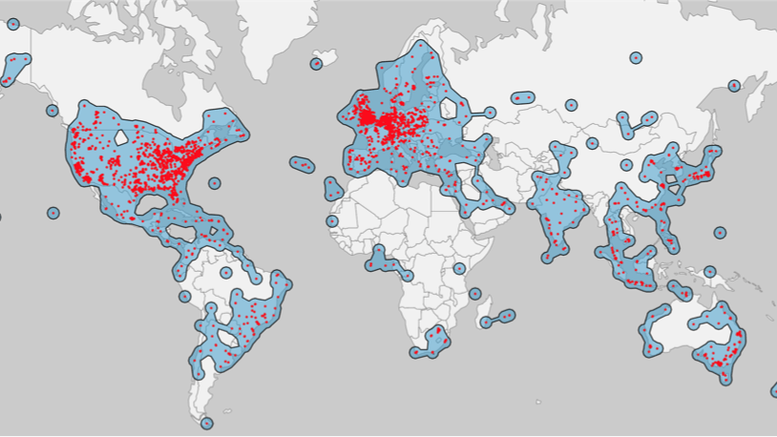
\includegraphics[width=14cm]{pic/1ADS-B-coverage.png}
\caption{全球陆基 ADS-B 覆盖情况}
\label{fig:1ADS-B-coverage}
\end{figure}

\subsection{澳大利亚}

ADS-B 地面站是视距(line-of-sight)设施\footnote{通常指波的传播路径为直线,不能沿曲线或者跨障碍物行进},地面站接收下行 ADS-B 数据的能力取决于飞机的高度、飞机与地面站的距离以及障碍物。在海拔较低的低空区域(接近地面),覆盖范围在距离地面站 20 海里半径内,高空空域覆盖半径可以超过 250 海里。

在雷达覆盖范围与 ADS-B 覆盖范围重叠的空域,雷达探测到的飞机位置将会提交给 ATC。

截至 2017 年 1 月,澳大利亚纯 ADS-B 覆盖区域如图\ref{fig:ADS-B-5000}、\ref{fig:ADS-B-10k}、\ref{fig:ADS-B-20k}、\ref{fig:ADS-B-30k}所示,澳大利亚 30000 英尺以上高空已实现 ADS-B 密集覆盖,航路管制间隔已缩至 5 海里水平。\footnote{数据来源:\url{http://www.airservicesaustralia.com/projects/ads-b/ads-b-coverage/}}

\begin{figure}[htbp]
\centering
\begin{minipage}[t]{0.48\textwidth}
\centering
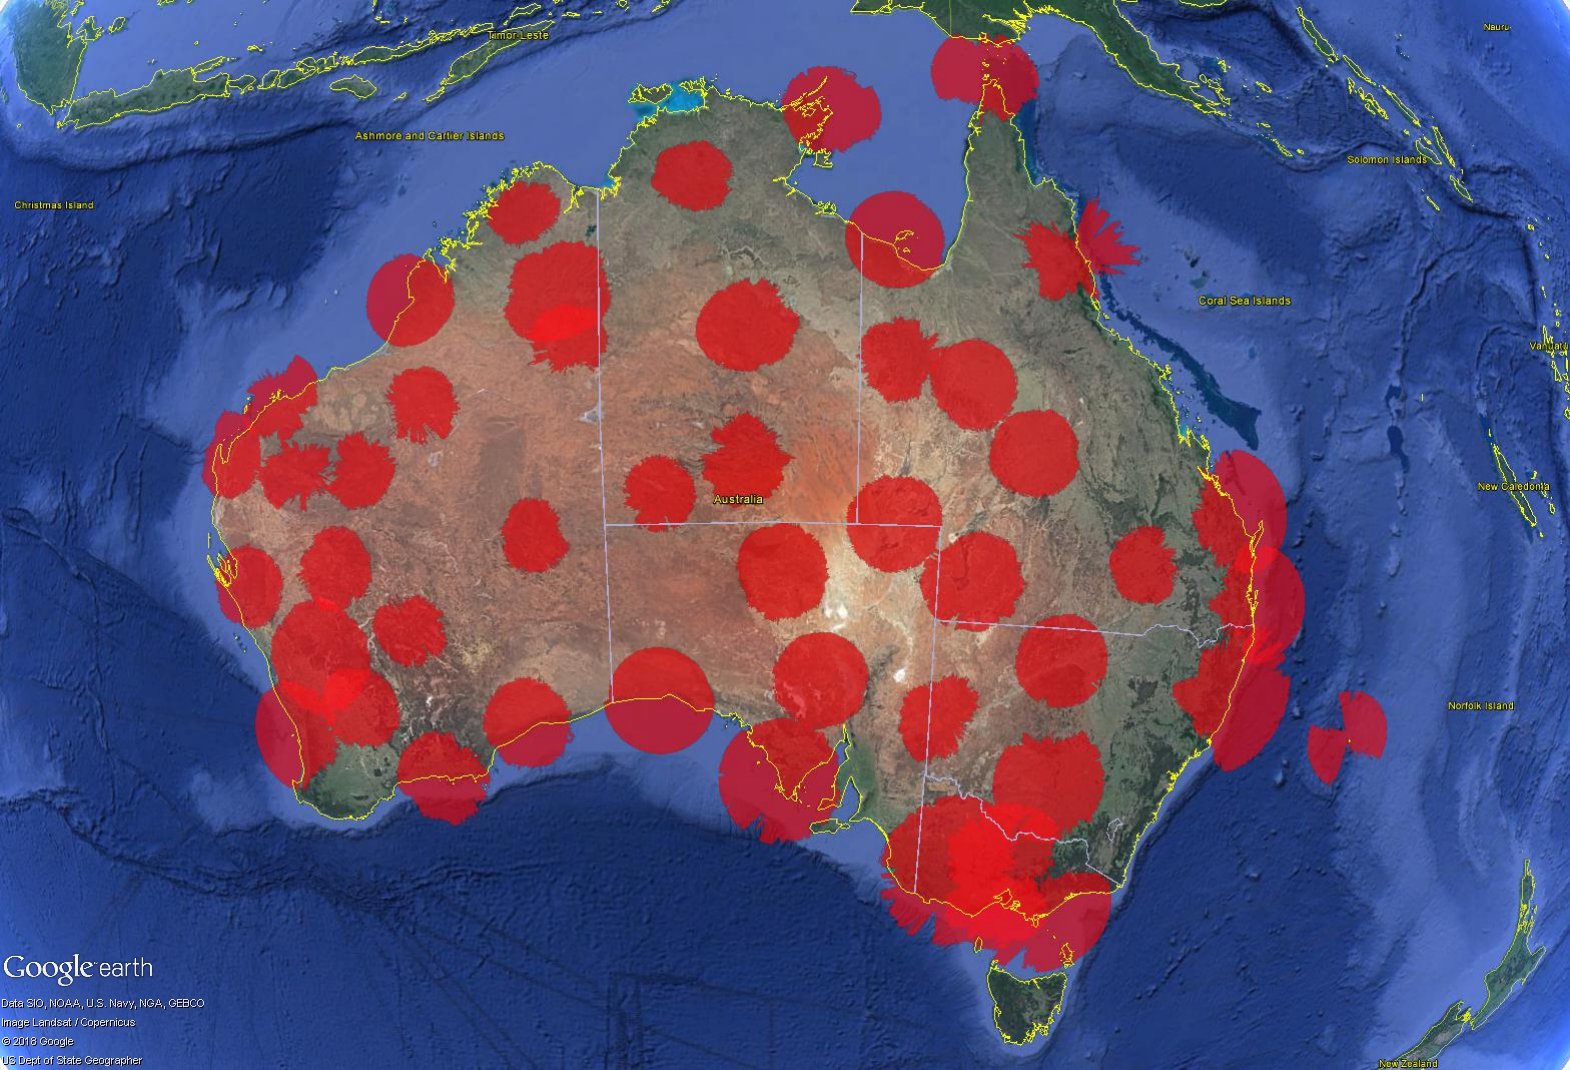
\includegraphics[width=7.5cm]{pic/ADS-B-5000.jpg}
\caption{澳洲 5000ft 空域覆盖范围}
\label{fig:ADS-B-5000}
\end{minipage}
\begin{minipage}[t]{0.48\textwidth}
\centering
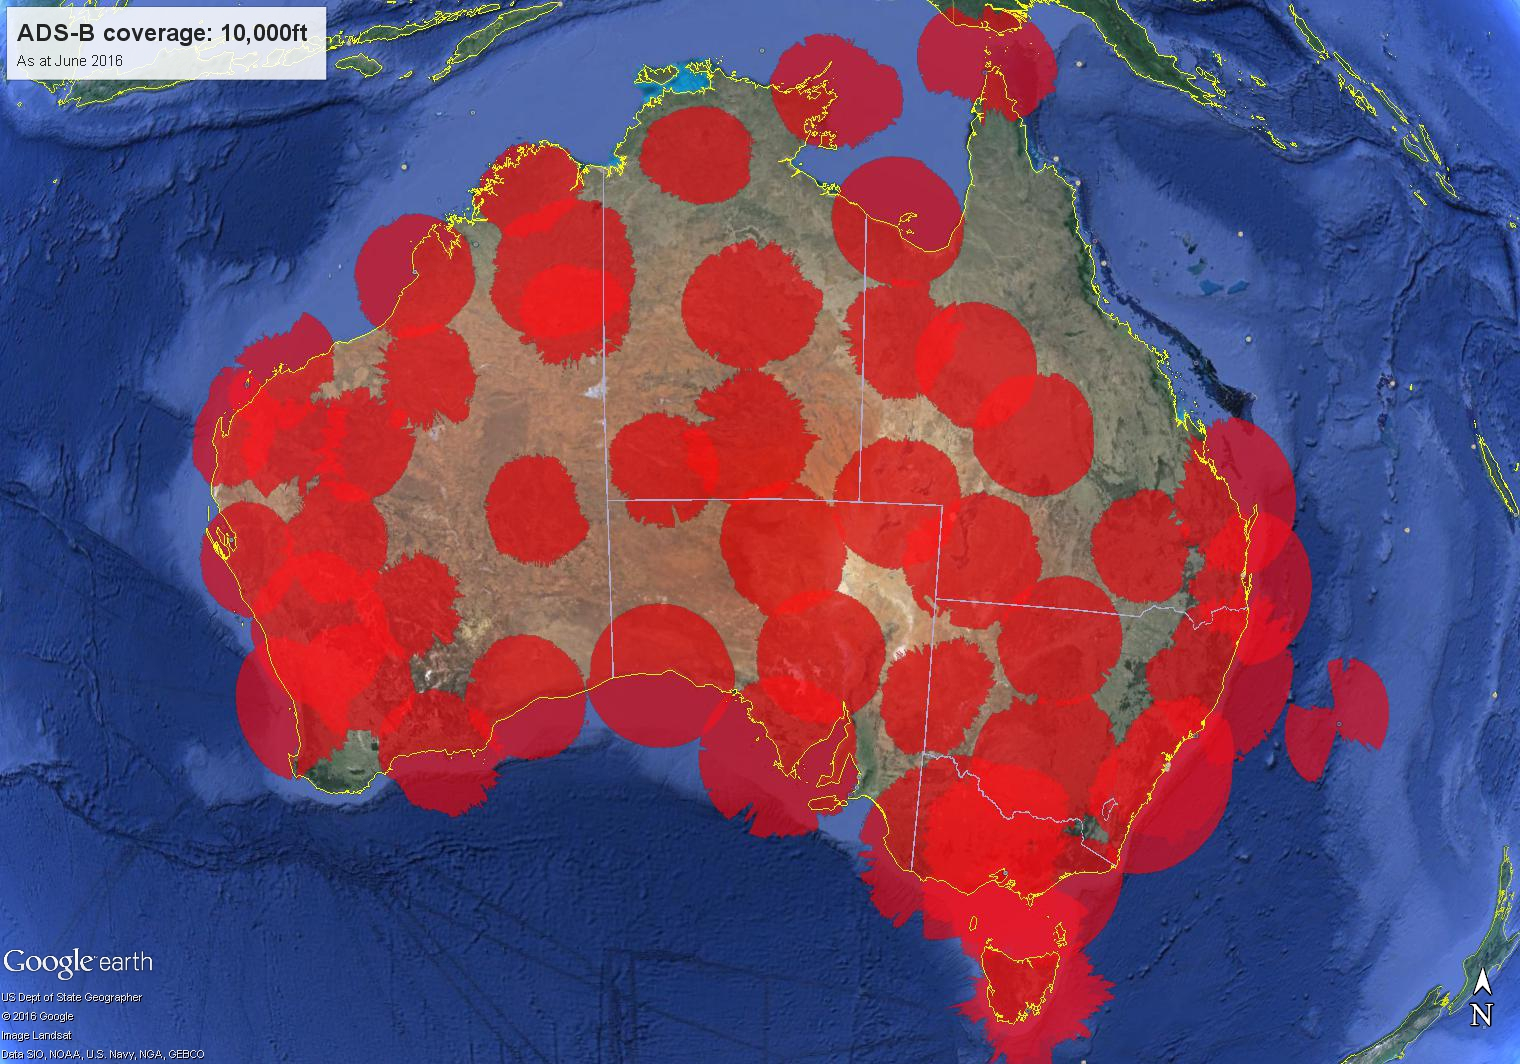
\includegraphics[width=7.5cm]{pic/ADS-B-10k.jpg}
\caption{澳洲 10000ft 空域覆盖范围}
\label{fig:ADS-B-10k}
\end{minipage}
\end{figure}

\begin{figure}[htbp]
\centering
\begin{minipage}[t]{0.48\textwidth}
\centering
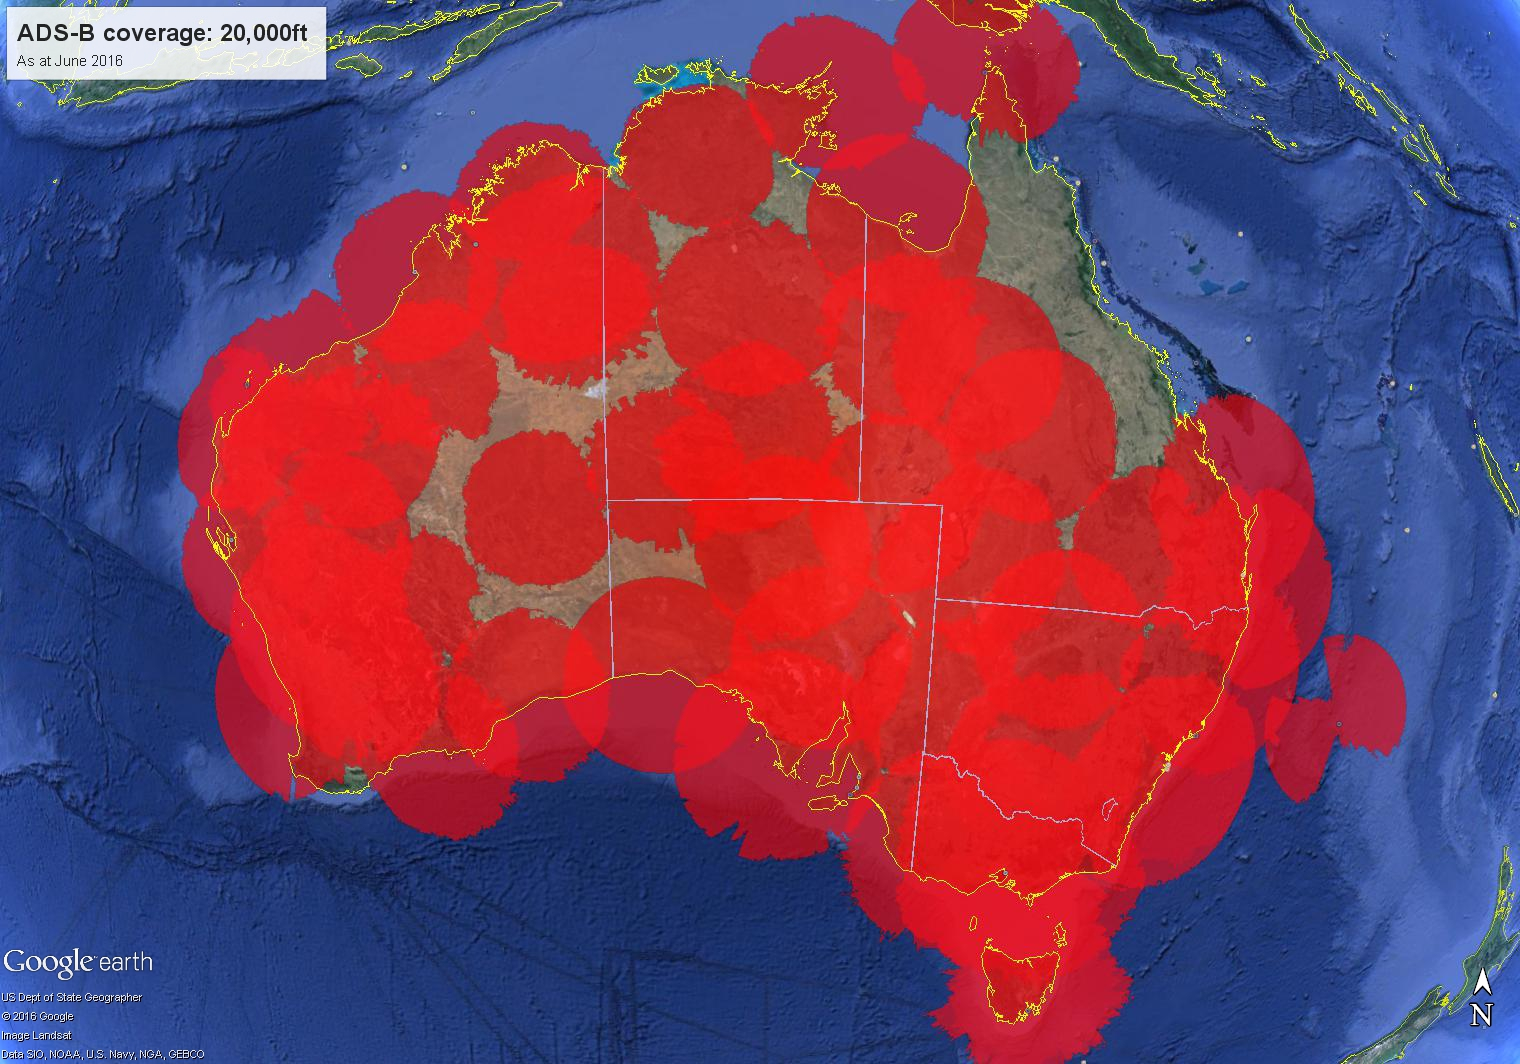
\includegraphics[width=7.5cm]{pic/ADS-B-20k.jpg}
\caption{澳洲 20000ft 空域覆盖范围}
\label{fig:ADS-B-20k}
\end{minipage}
\begin{minipage}[t]{0.48\textwidth}
\centering
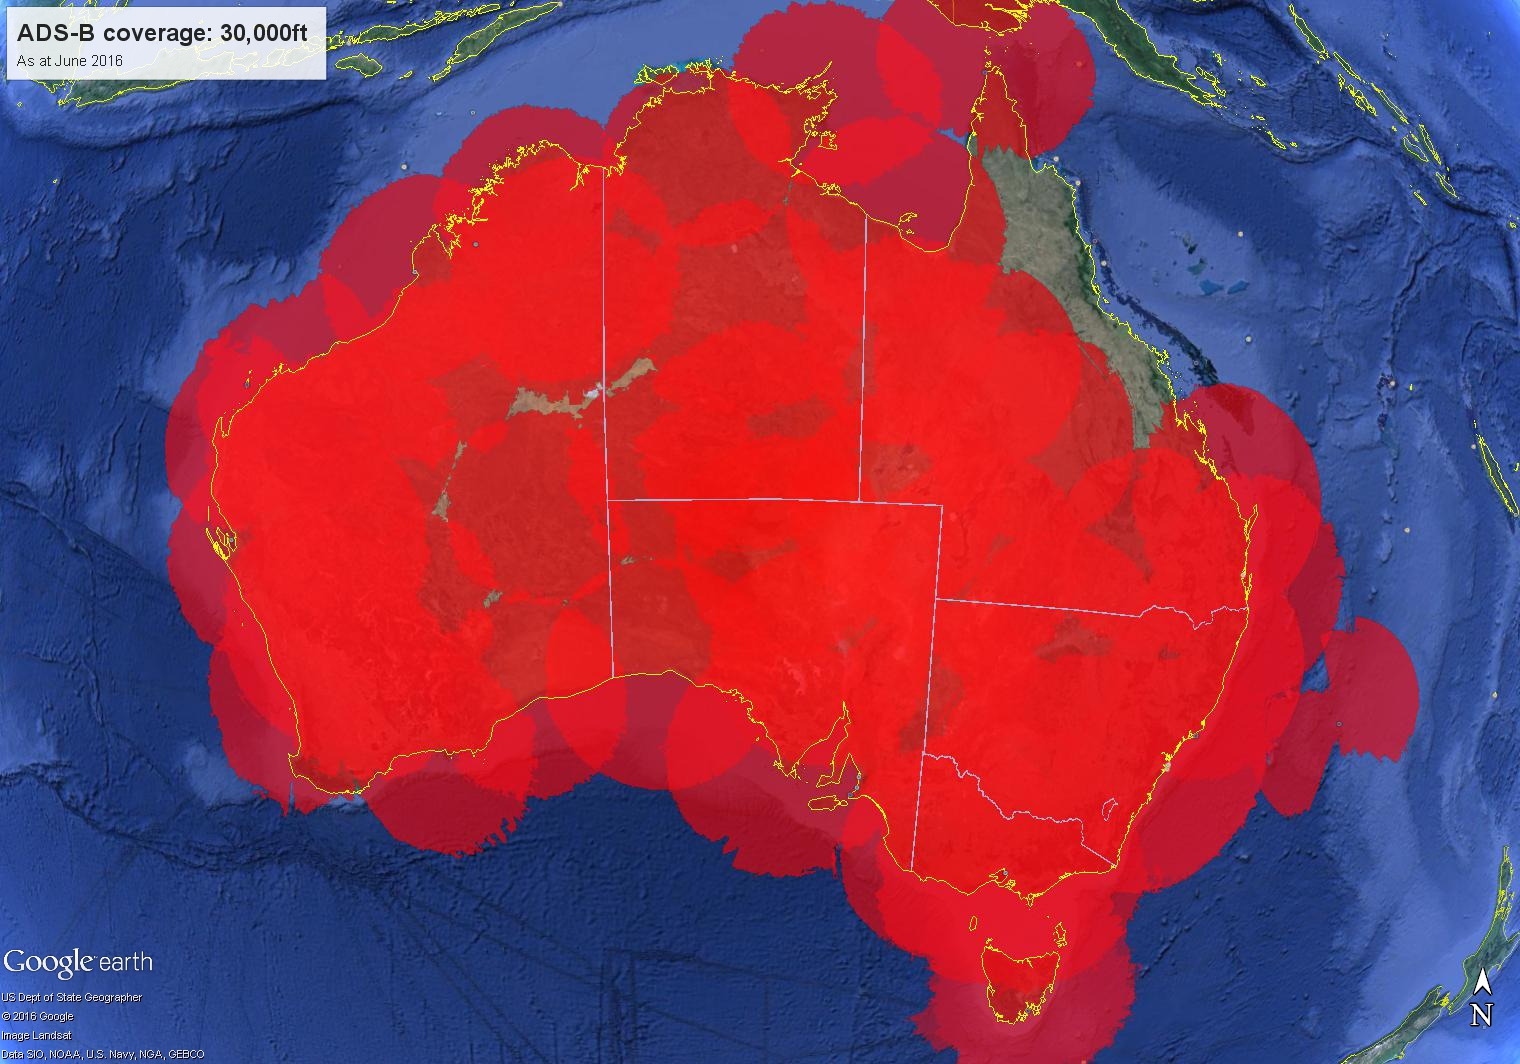
\includegraphics[width=7.5cm]{pic/ADS-B-30k.jpg}
\caption{澳洲 30000ft 空域覆盖范围}
\label{fig:ADS-B-30k}
\end{minipage}
\end{figure}

\subsection{北美地区}

截至 2017 年 4 月,ADS-B 在美国全境的覆盖情况如图\ref{fig:ADS-B-Coverage-Area}所示。\footnote{数据来源:Corporate Fleet Service(CFS),\url{http://cfsjets.com/2017/12/14/ads-b-where-we-are-now//}}

\begin{figure}[htbp]
\centering
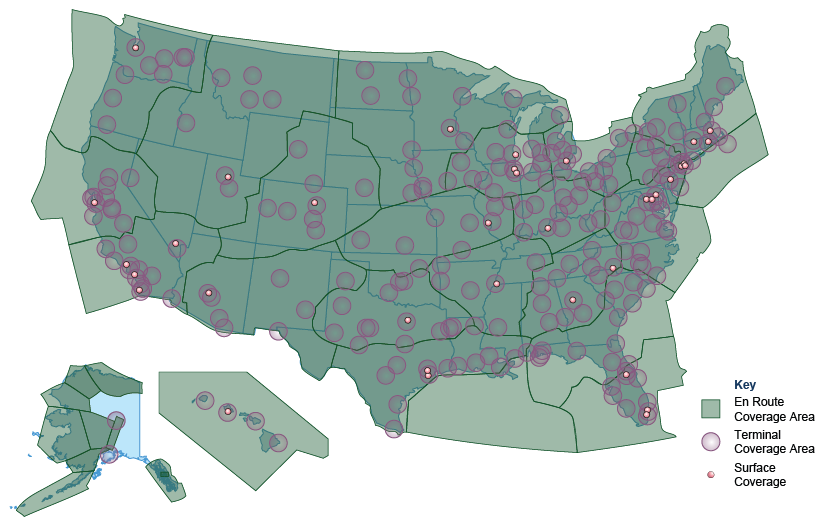
\includegraphics[width=14cm]{pic/ADS-B-Coverage-Area.png}
\caption{美国陆基 ADS-B 覆盖情况}
\label{fig:ADS-B-Coverage-Area}
\end{figure}

\begin{figure}[htbp]
\centering
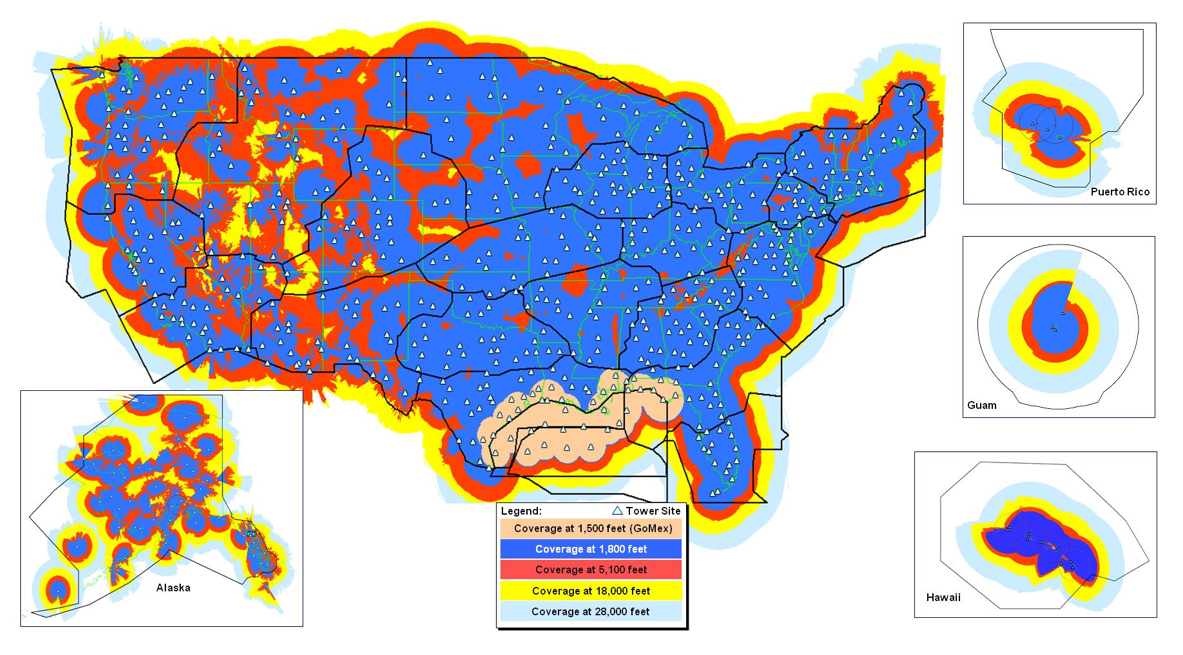
\includegraphics[width=14cm]{pic/ADSB-final.png}
\caption{美国不同高度层 ADS-B 覆盖情况}
\label{fig:ADSB-final}
\end{figure}

更为详细的 ADS-B 覆盖情况可以在 FAA 网站\footnote{\url{https://www.faa.gov/nextgen/programs/adsb/}}上查询,它提供了一个动态的可交互式的 ADS-B 覆盖范围查询网页。

\subsection{欧洲}

\begin{figure}[htbp]
\centering
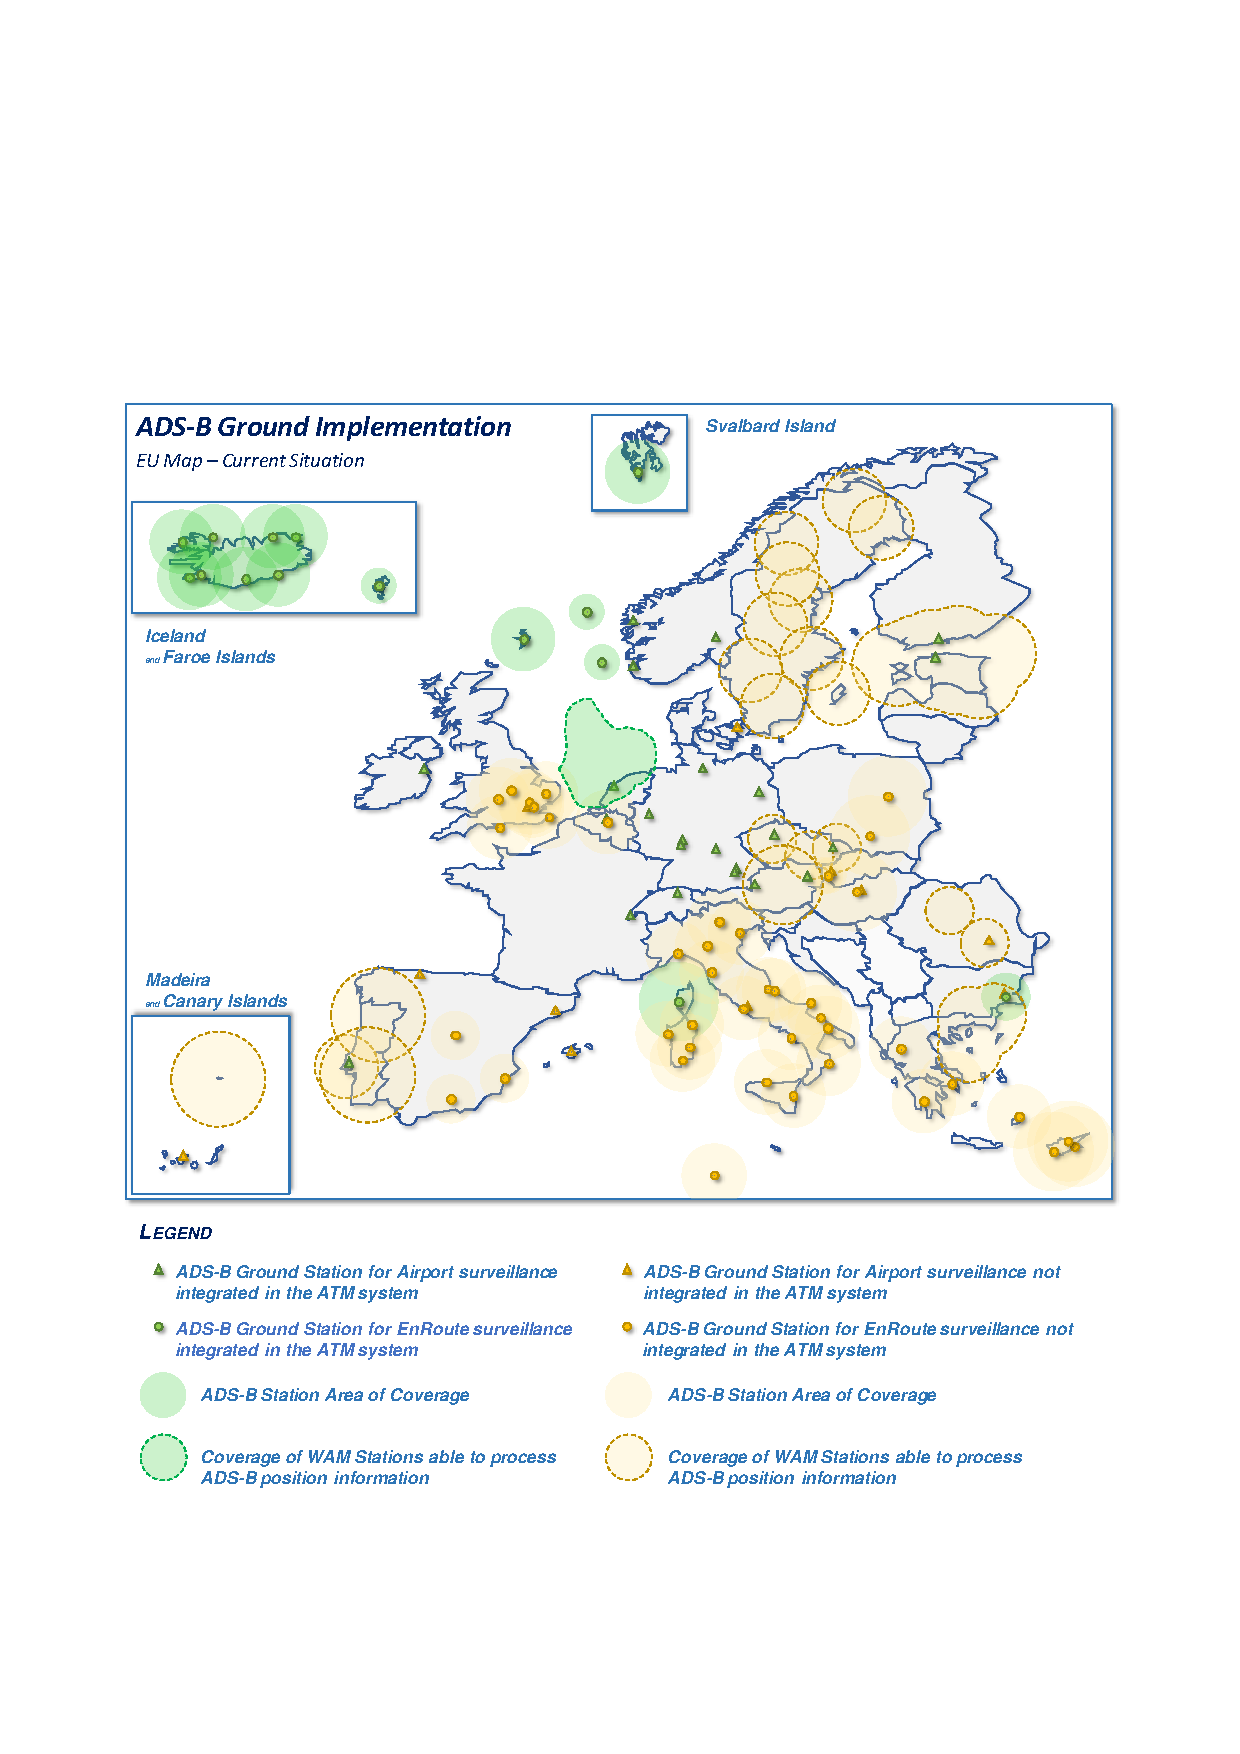
\includegraphics[width=10cm]{pic/20180515-sesar-ads-b-report_18.pdf}
\caption{欧洲 1}
\label{fig:20180515-sesar-ads-b-report_18}
\end{figure}

\begin{figure}[htbp]
\centering
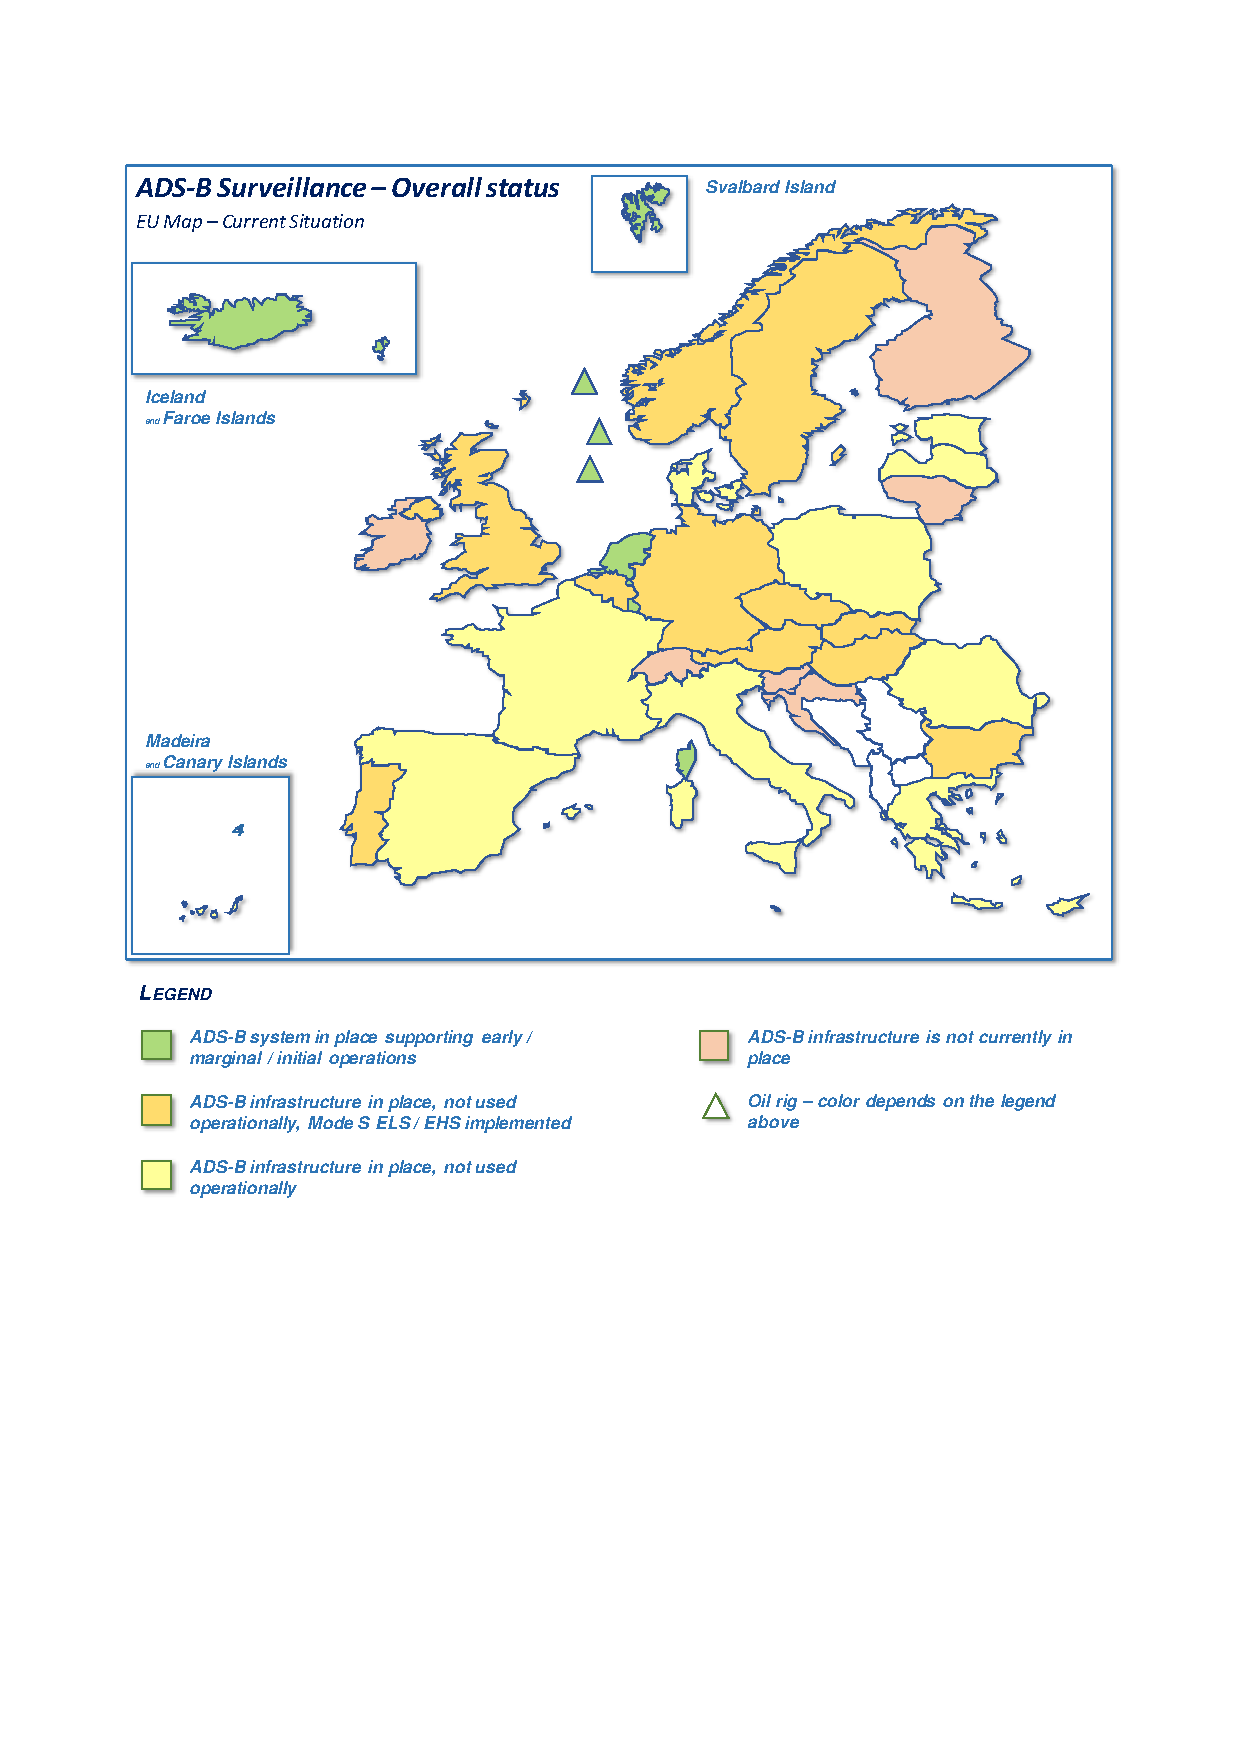
\includegraphics[width=10cm]{pic/20180515-sesar-ads-b-report_23.pdf}
\caption{欧洲 2}
\label{fig:20180515-sesar-ads-b-report_23}
\end{figure}

\begin{figure}[htbp]
\centering
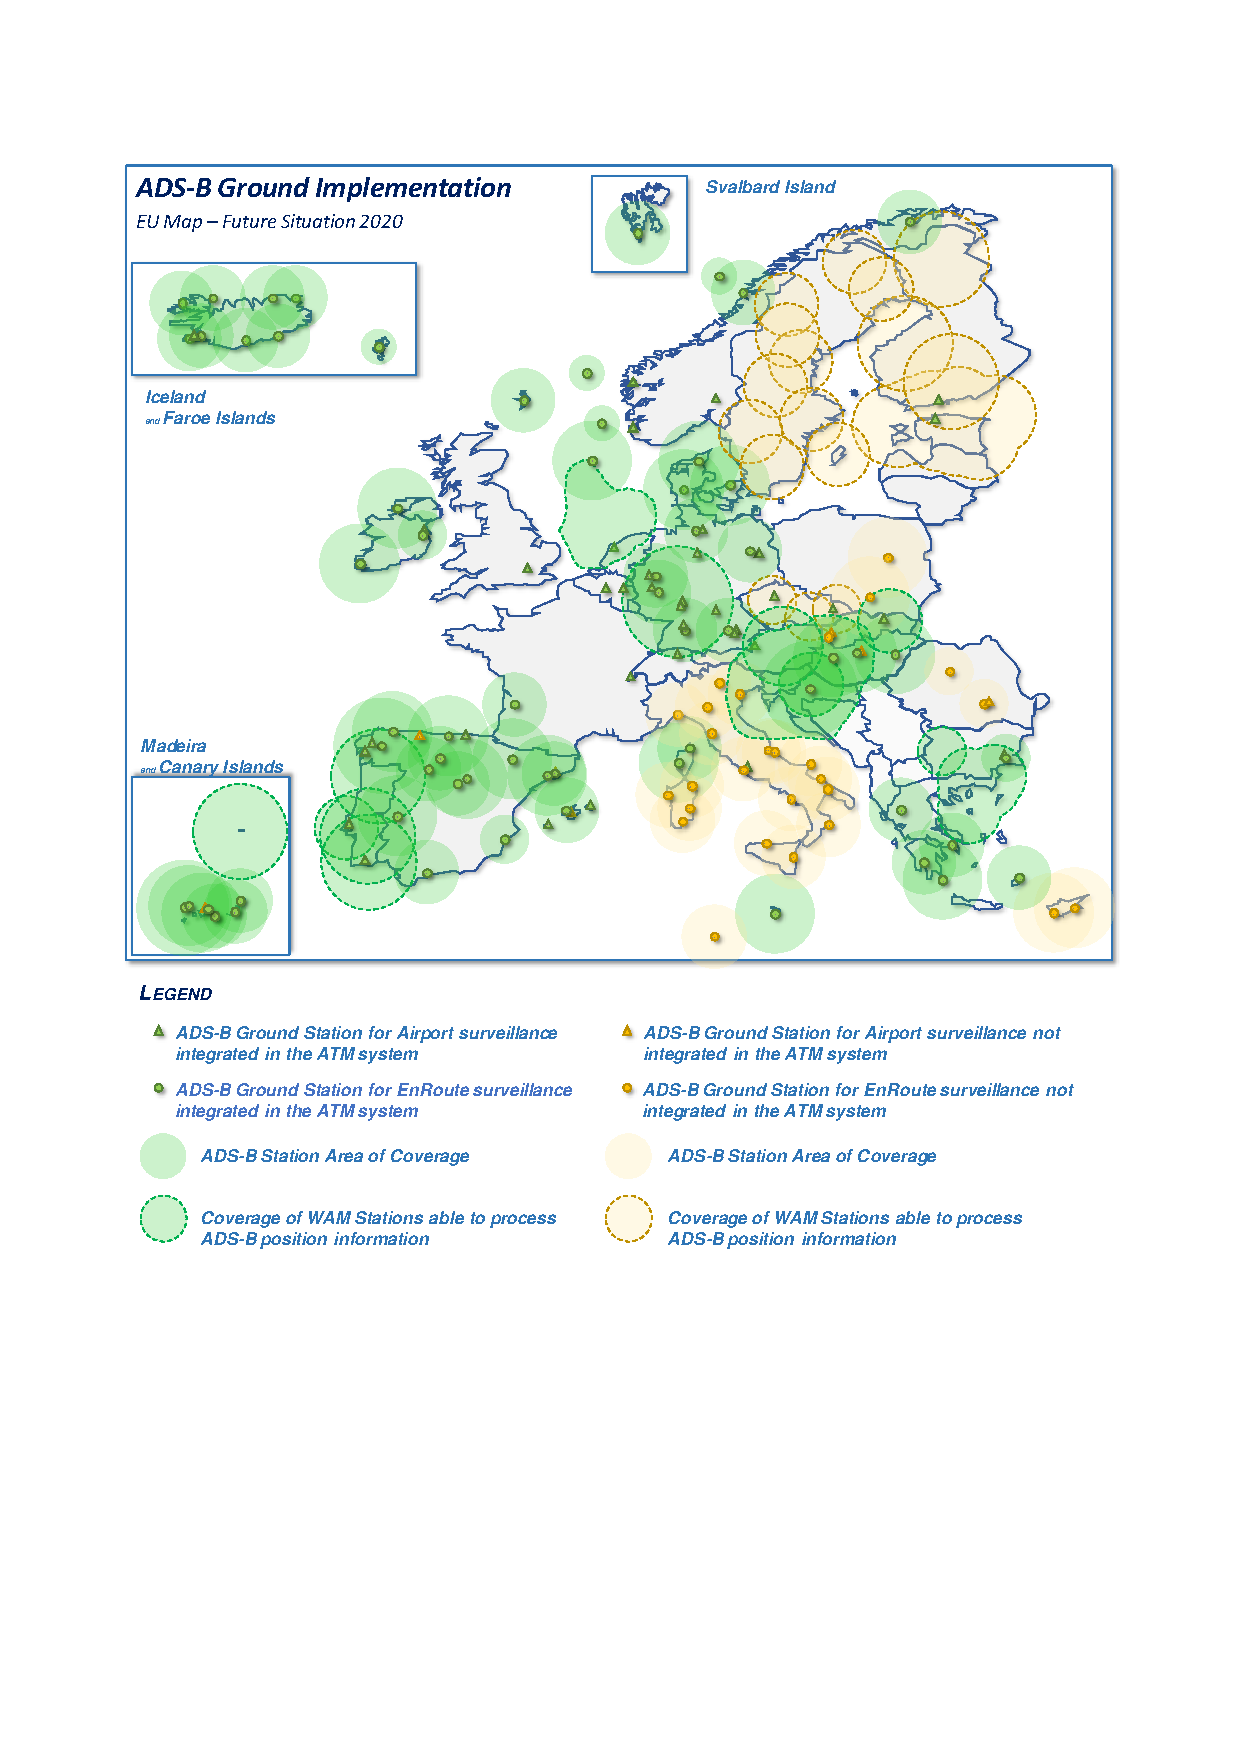
\includegraphics[width=10cm]{pic/20180515-sesar-ads-b-report_33.pdf}
\caption{欧洲 3}
\label{fig:20180515-sesar-ads-b-report_33}
\end{figure}

\begin{figure}[htbp]
\centering
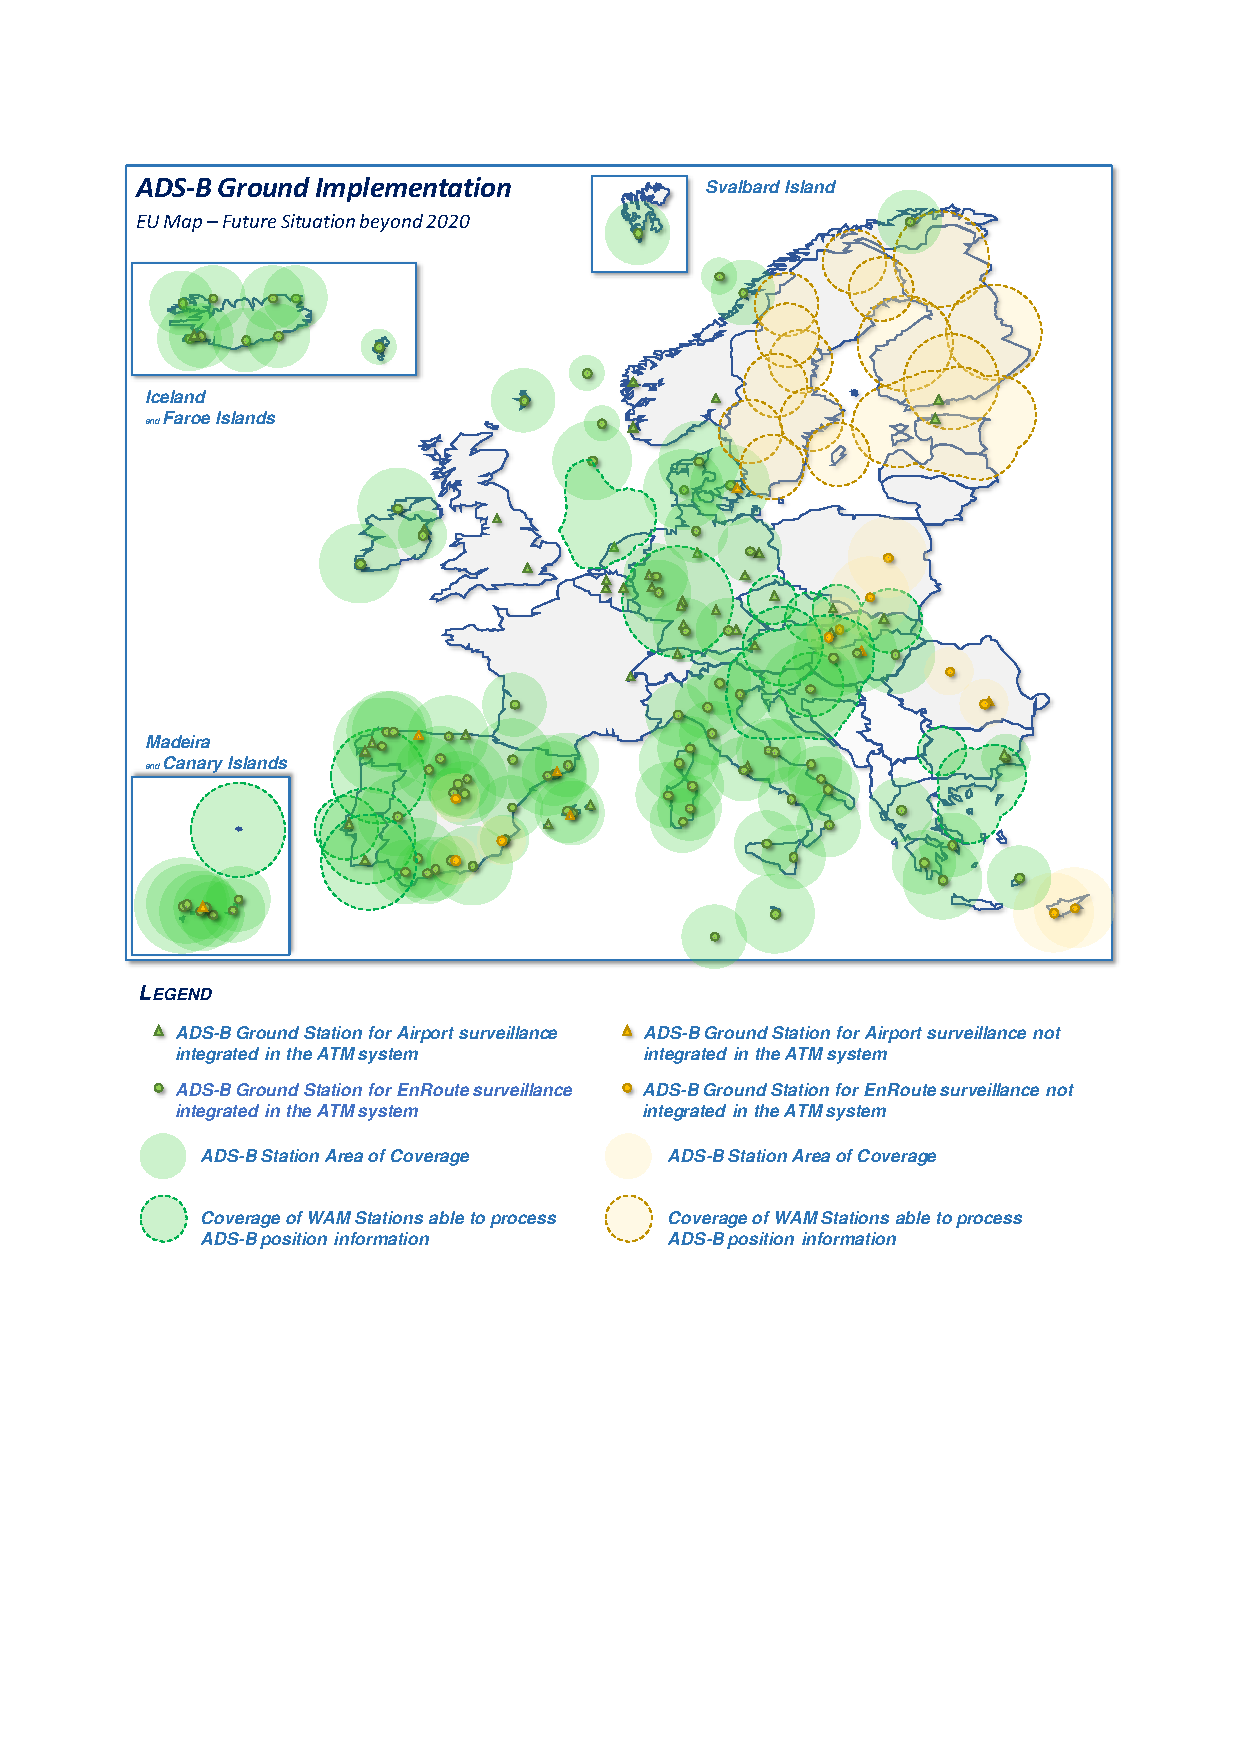
\includegraphics[width=10cm]{pic/20180515-sesar-ads-b-report_35.pdf}
\caption{欧洲 4}
\label{fig:20180515-sesar-ads-b-report_35}
\end{figure}

\begin{figure}[htbp]
\centering
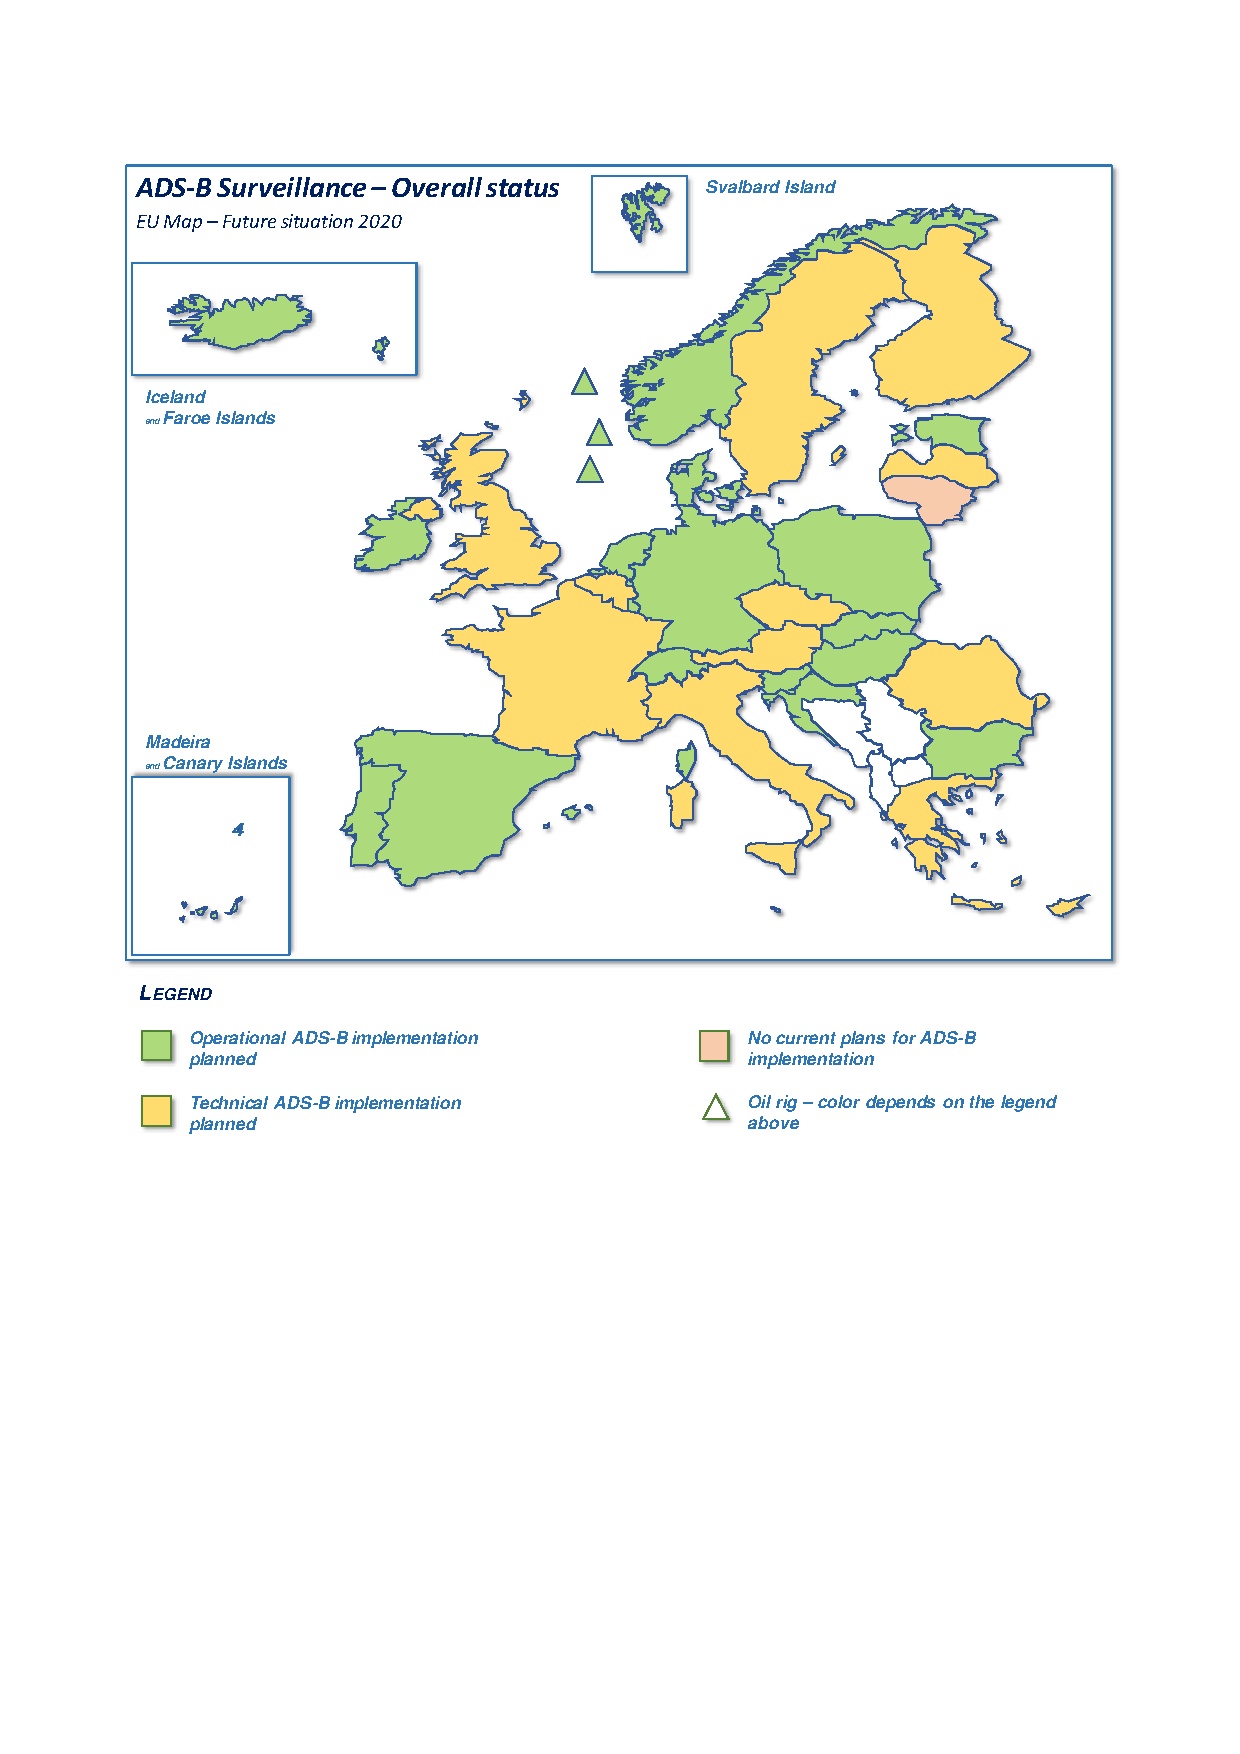
\includegraphics[width=10cm]{pic/20180515-sesar-ads-b-report_39.pdf}
\caption{欧洲 5}
\label{fig:20180515-sesar-ads-b-report_39}
\end{figure}

\begin{figure}[htbp]
\centering
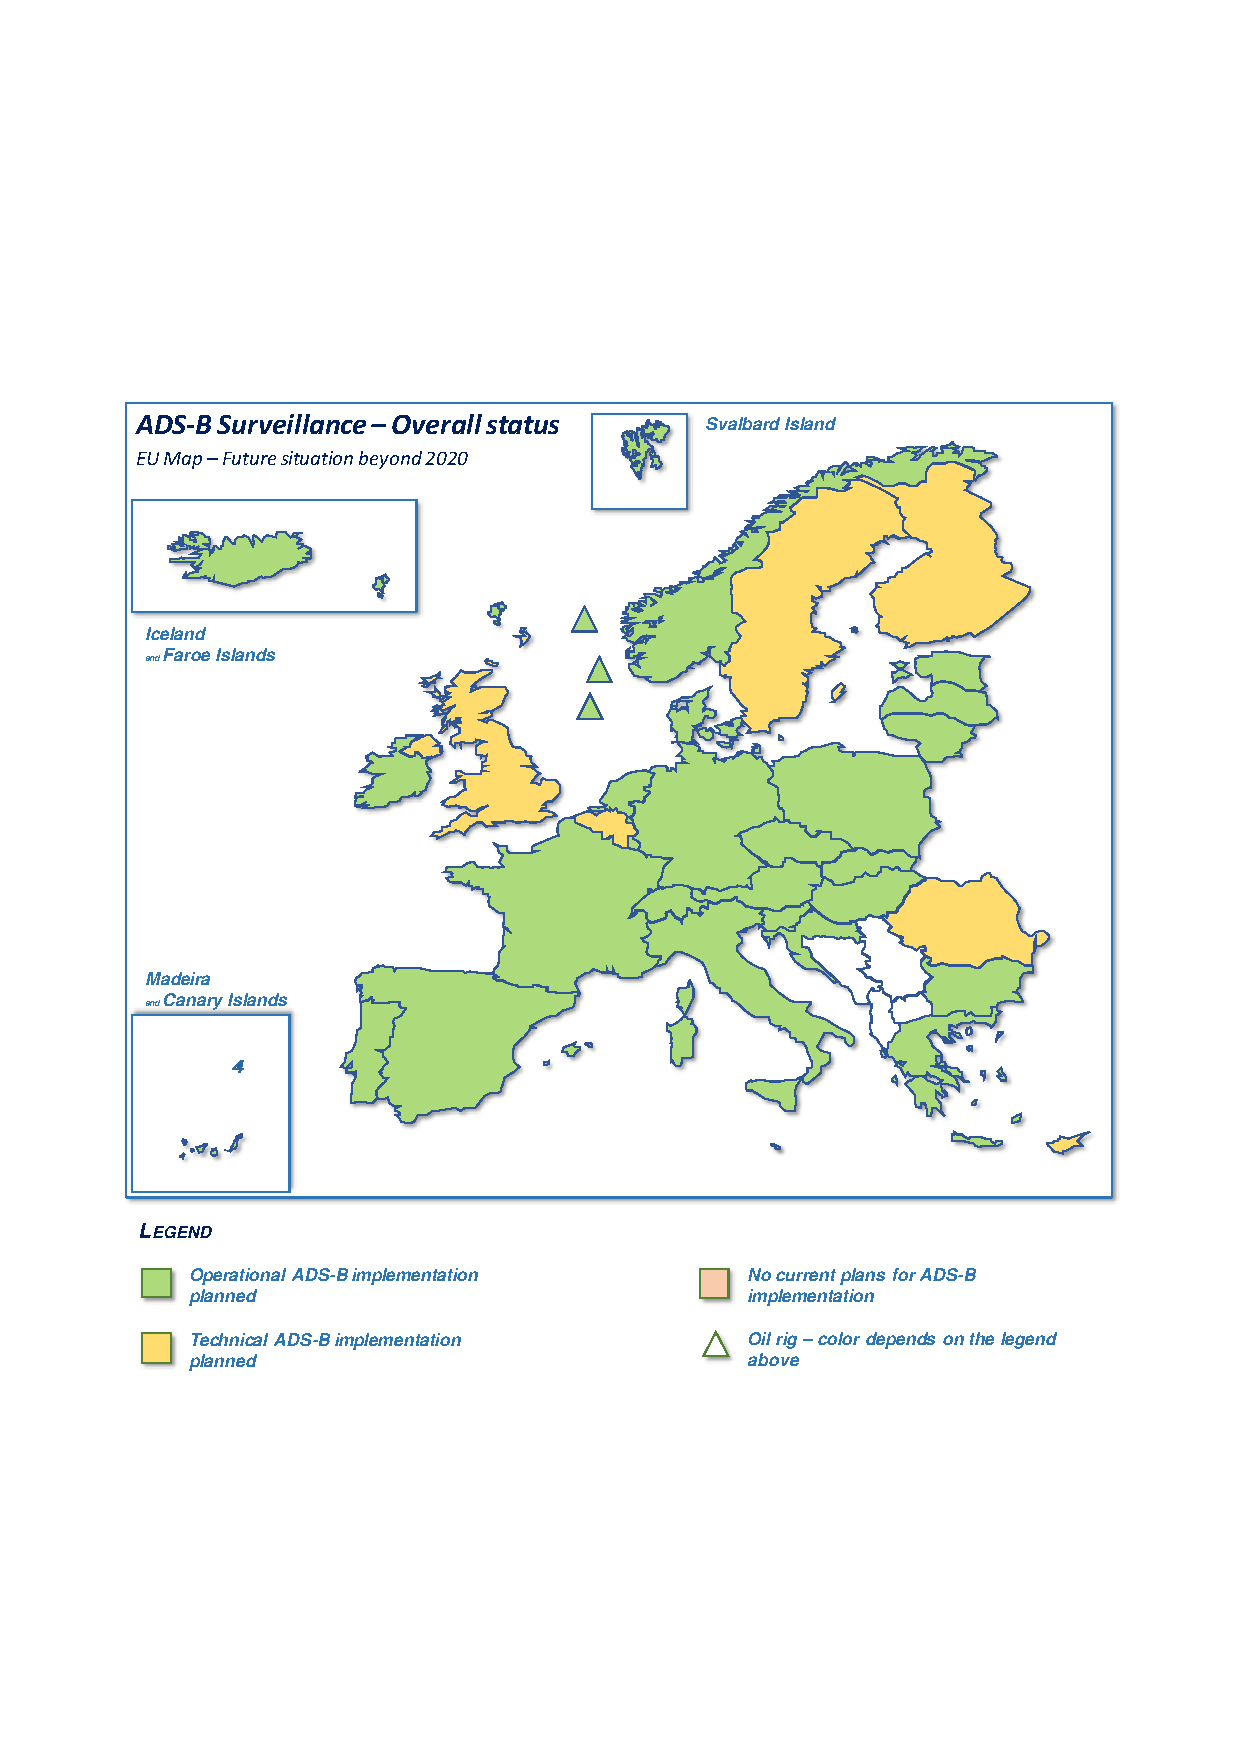
\includegraphics[width=10cm]{pic/20180515-sesar-ads-b-report_40.pdf}
\caption{欧洲 6}
\label{fig:20180515-sesar-ads-b-report_40}
\end{figure}

\subsection{中国}

\begin{figure}[htbp]
\centering
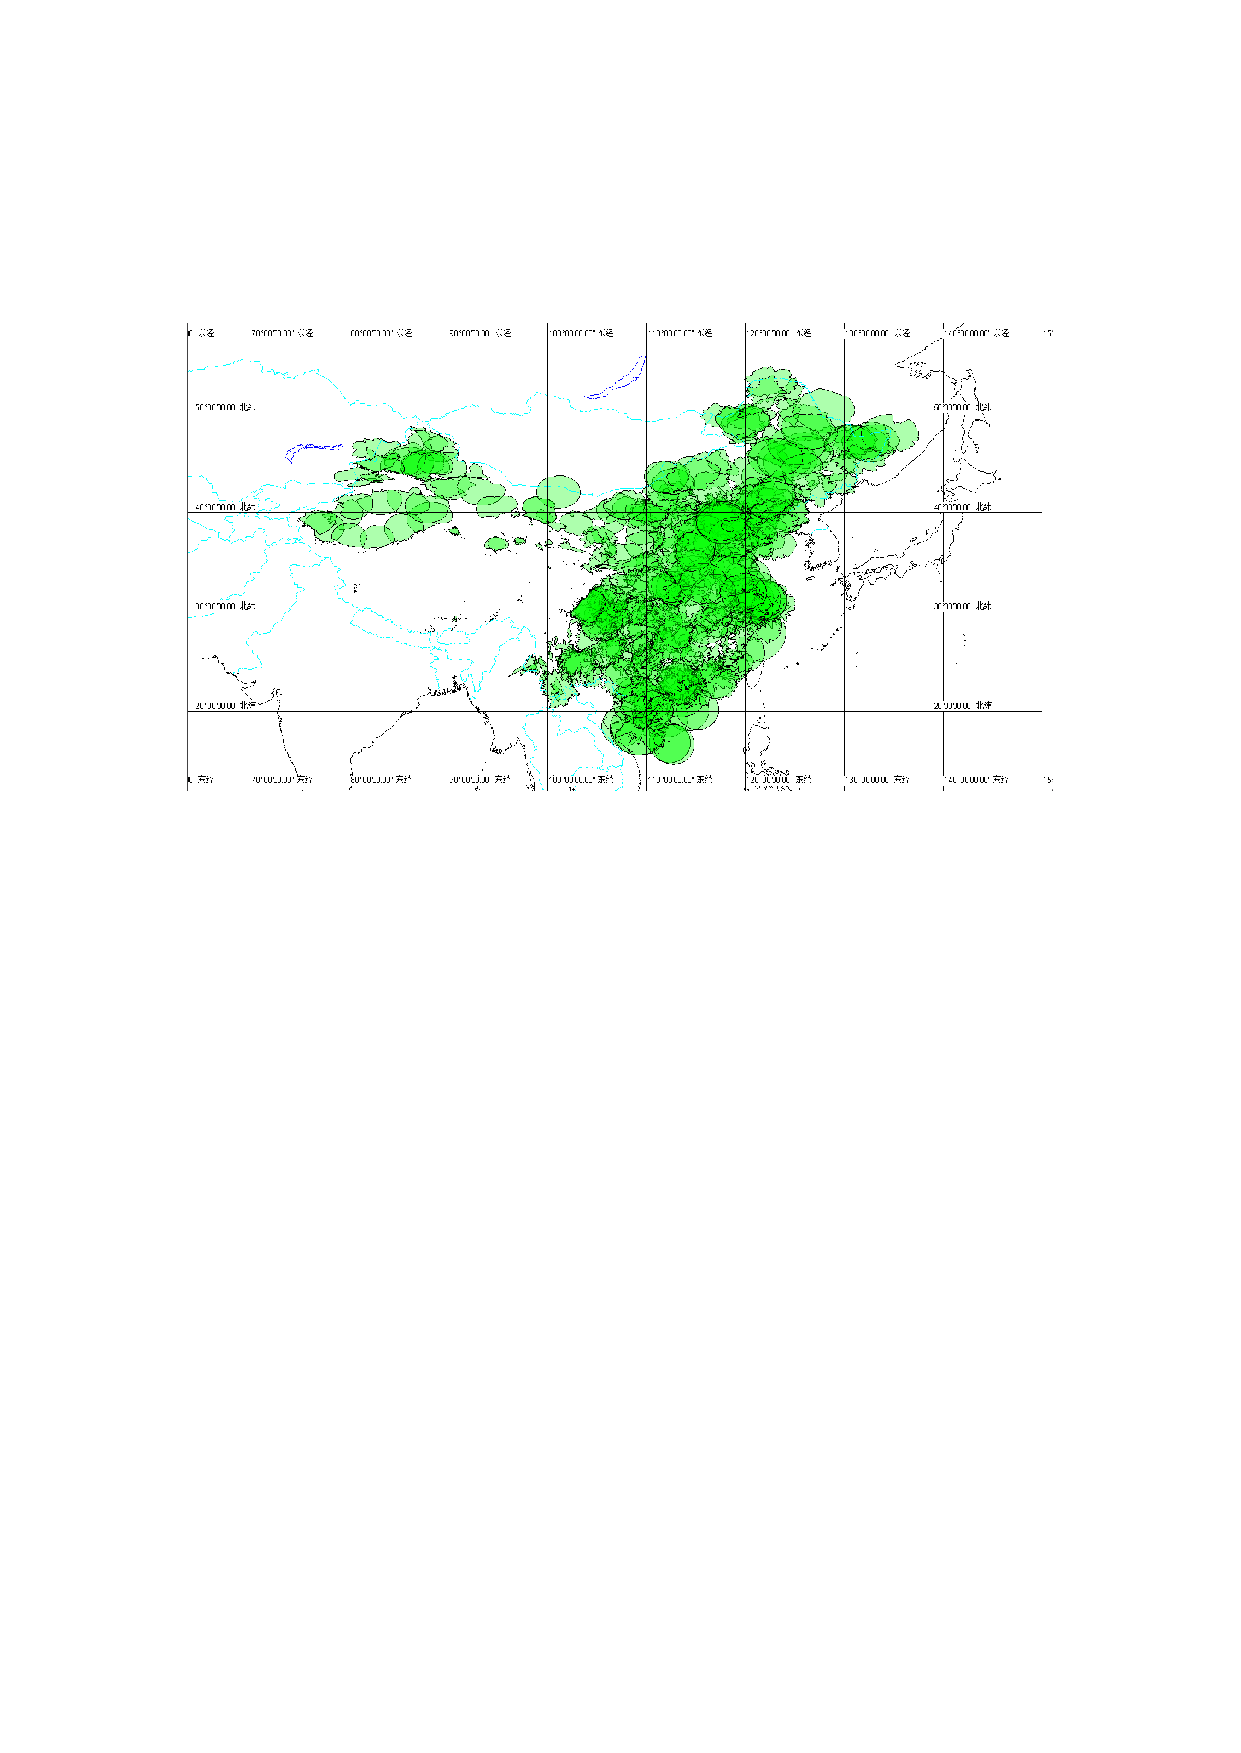
\includegraphics[width=12cm]{pic/china_3300m.pdf}
\caption{中国 3300m }
\label{fig:china_3300m}
\end{figure}

\begin{figure}[htbp]
\centering
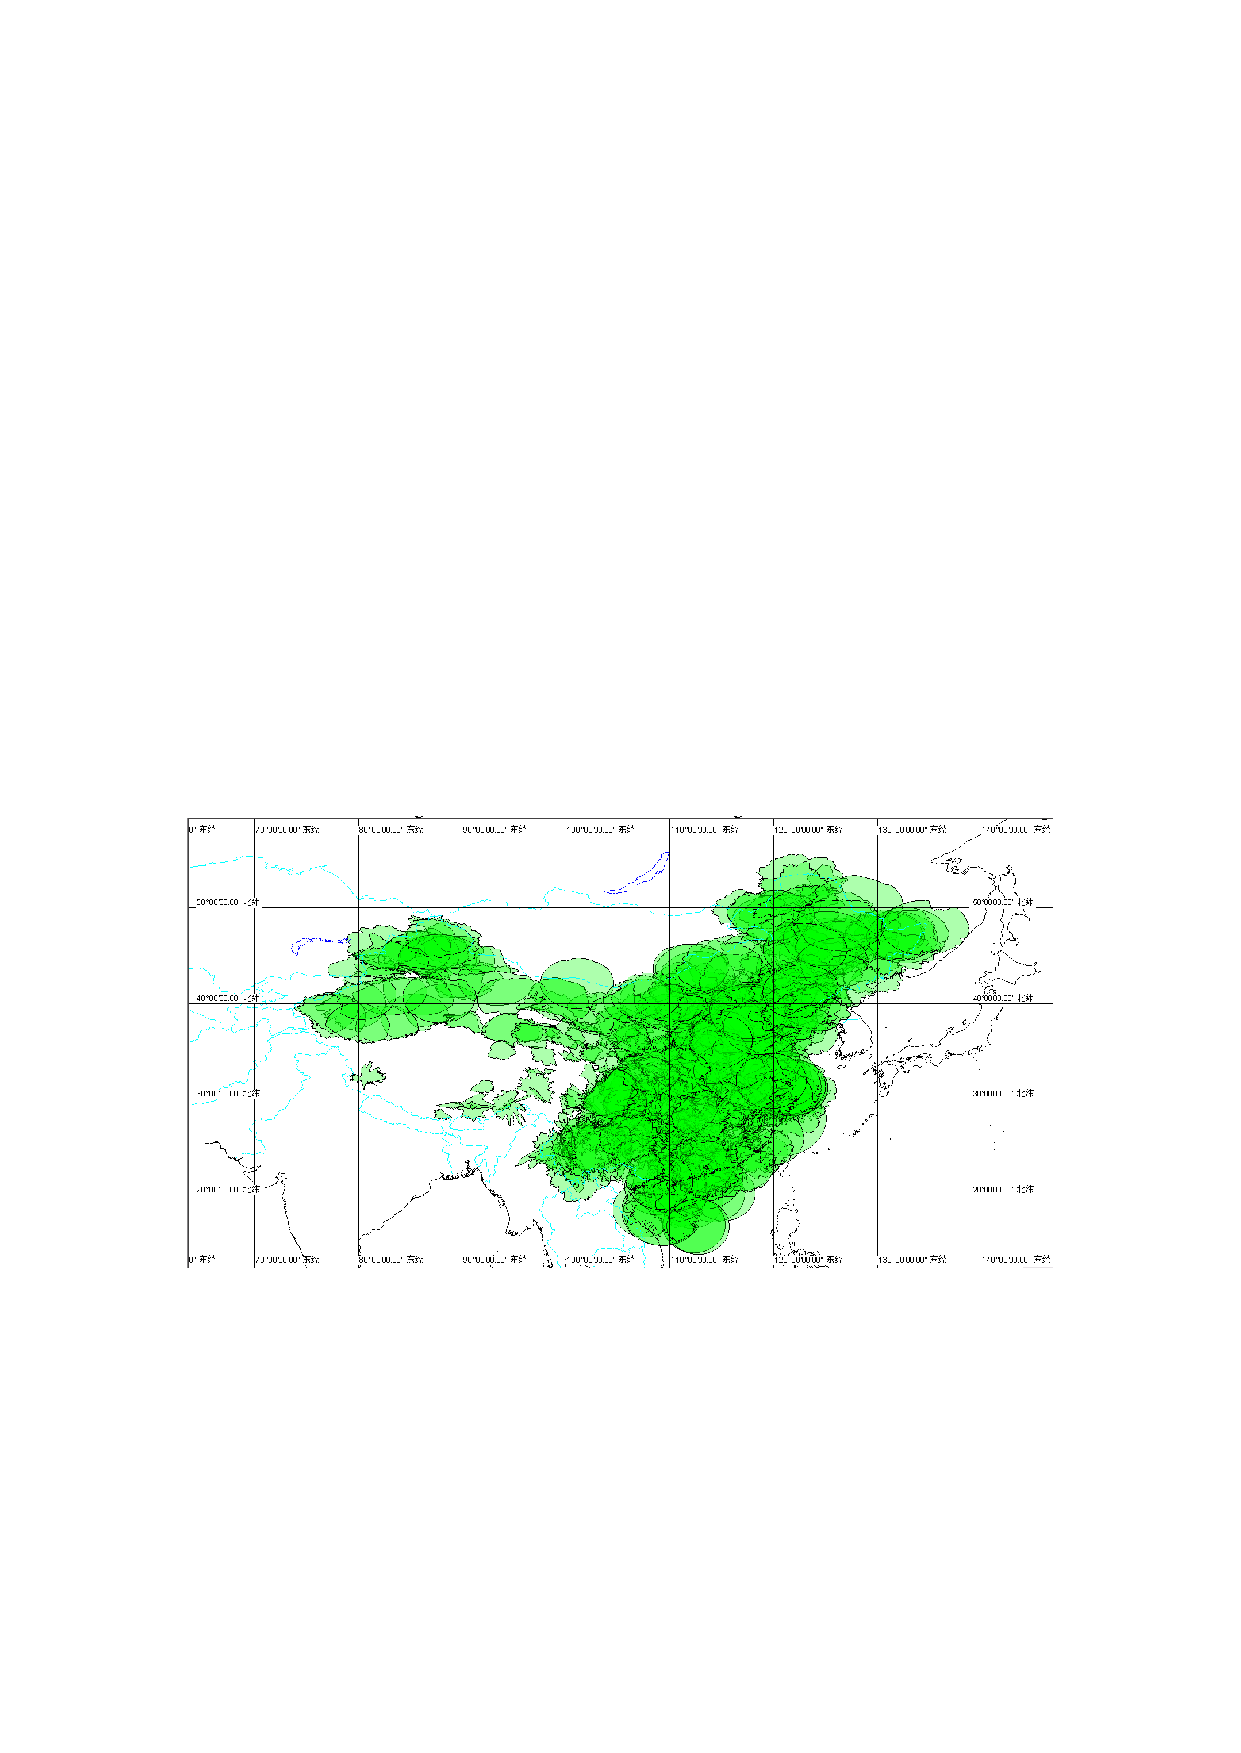
\includegraphics[width=12cm]{pic/china_6600m.pdf}
\caption{中国 6600m }
\label{fig:china_6600m}
\end{figure}

\begin{figure}[htbp]
\centering
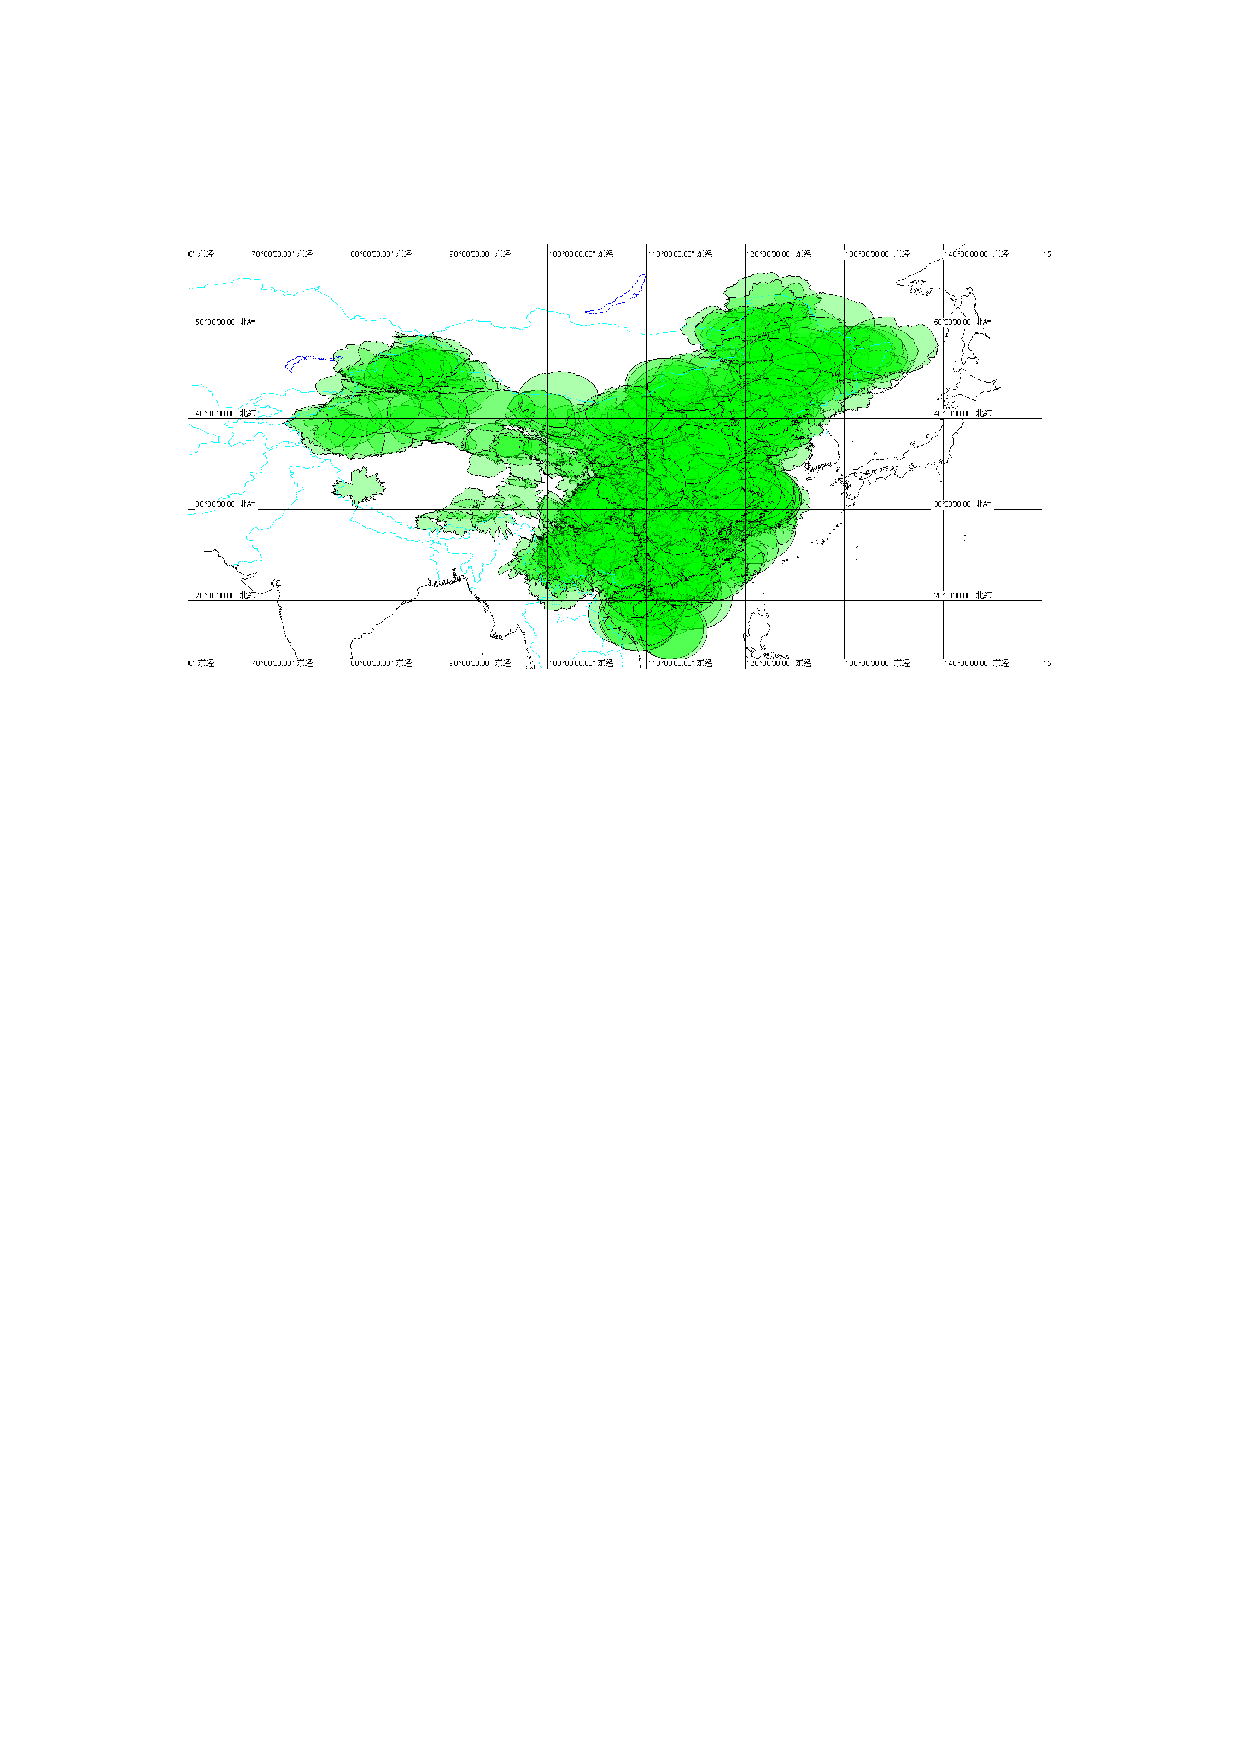
\includegraphics[width=12cm]{pic/china_8400m.pdf}
\caption{中国 8400m }
\label{fig:china_8400m}
\end{figure}

\subsection{东南亚}

\subsubsection{马来西亚}

\begin{figure}[htbp]
\centering
\begin{minipage}[t]{0.48\textwidth}
\centering
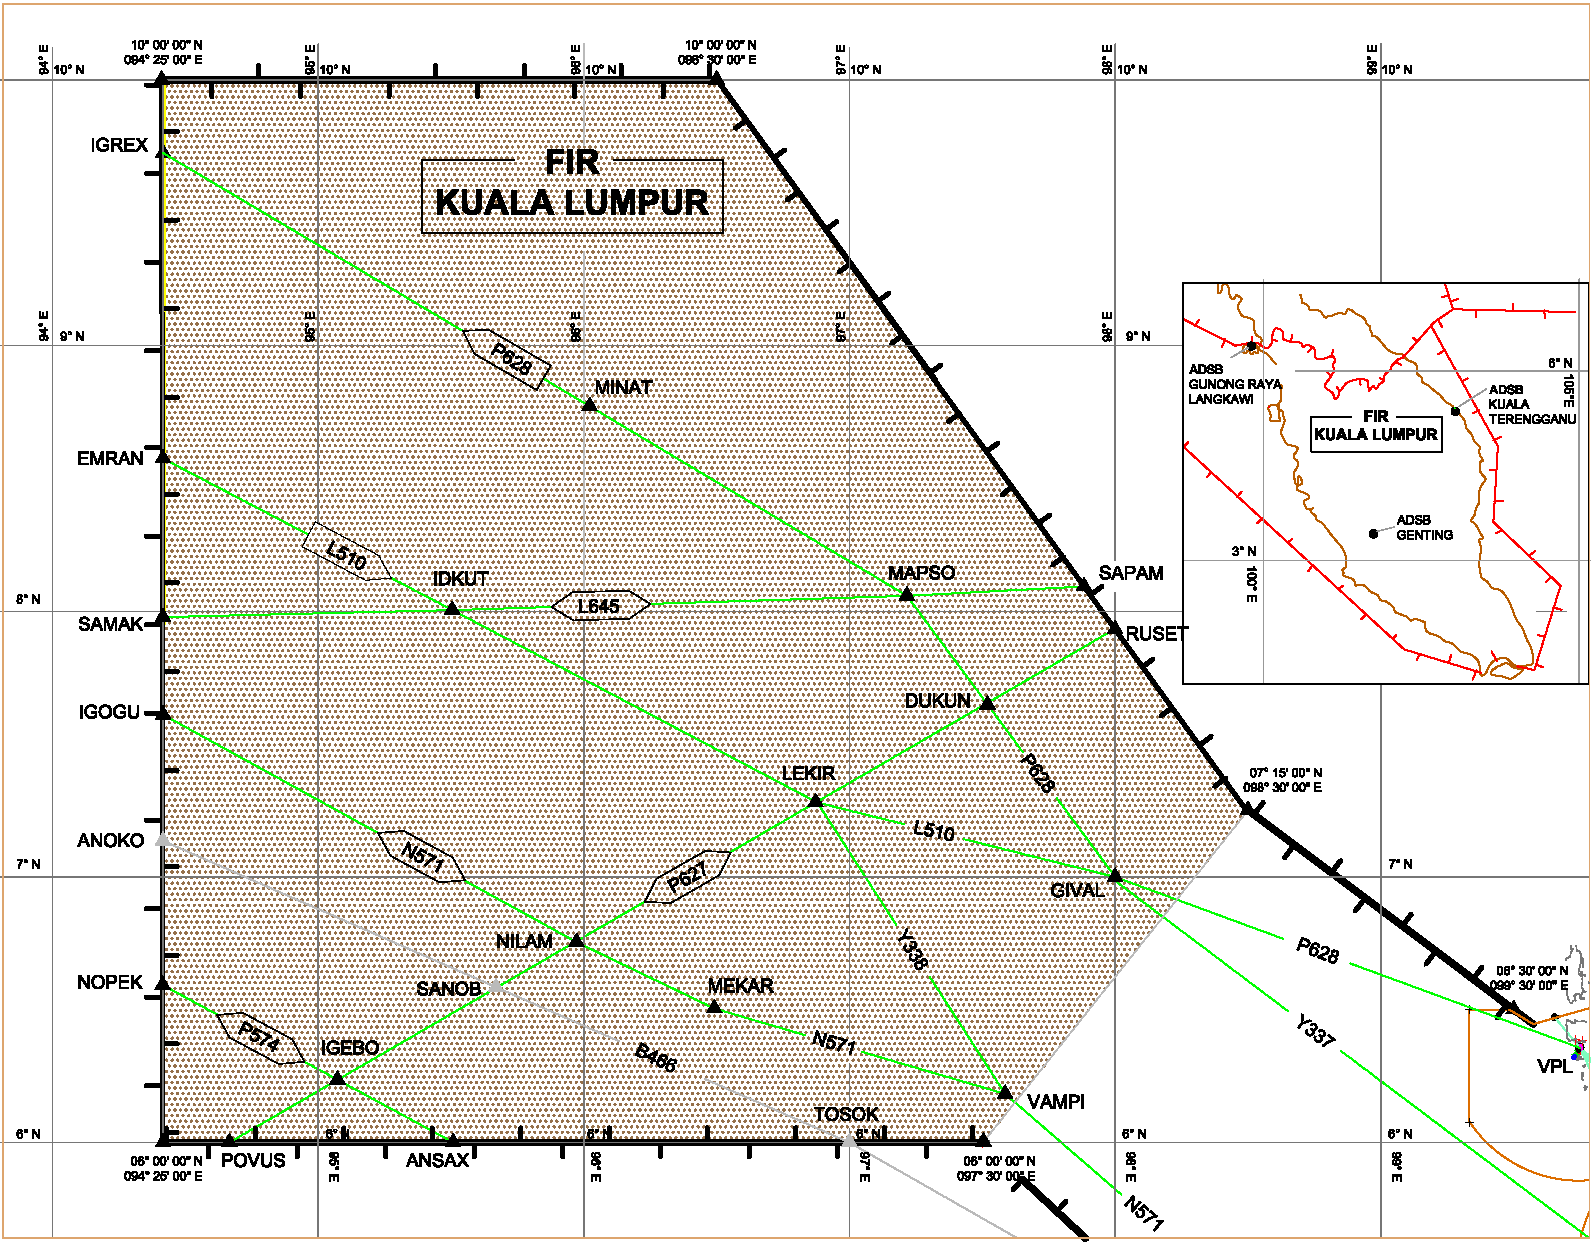
\includegraphics[width=8cm]{pic/malaysia_cover.png}
\caption{马来西亚}
\label{fig:malaysia_cover}
\end{minipage}
\begin{minipage}[t]{0.48\textwidth}
\centering
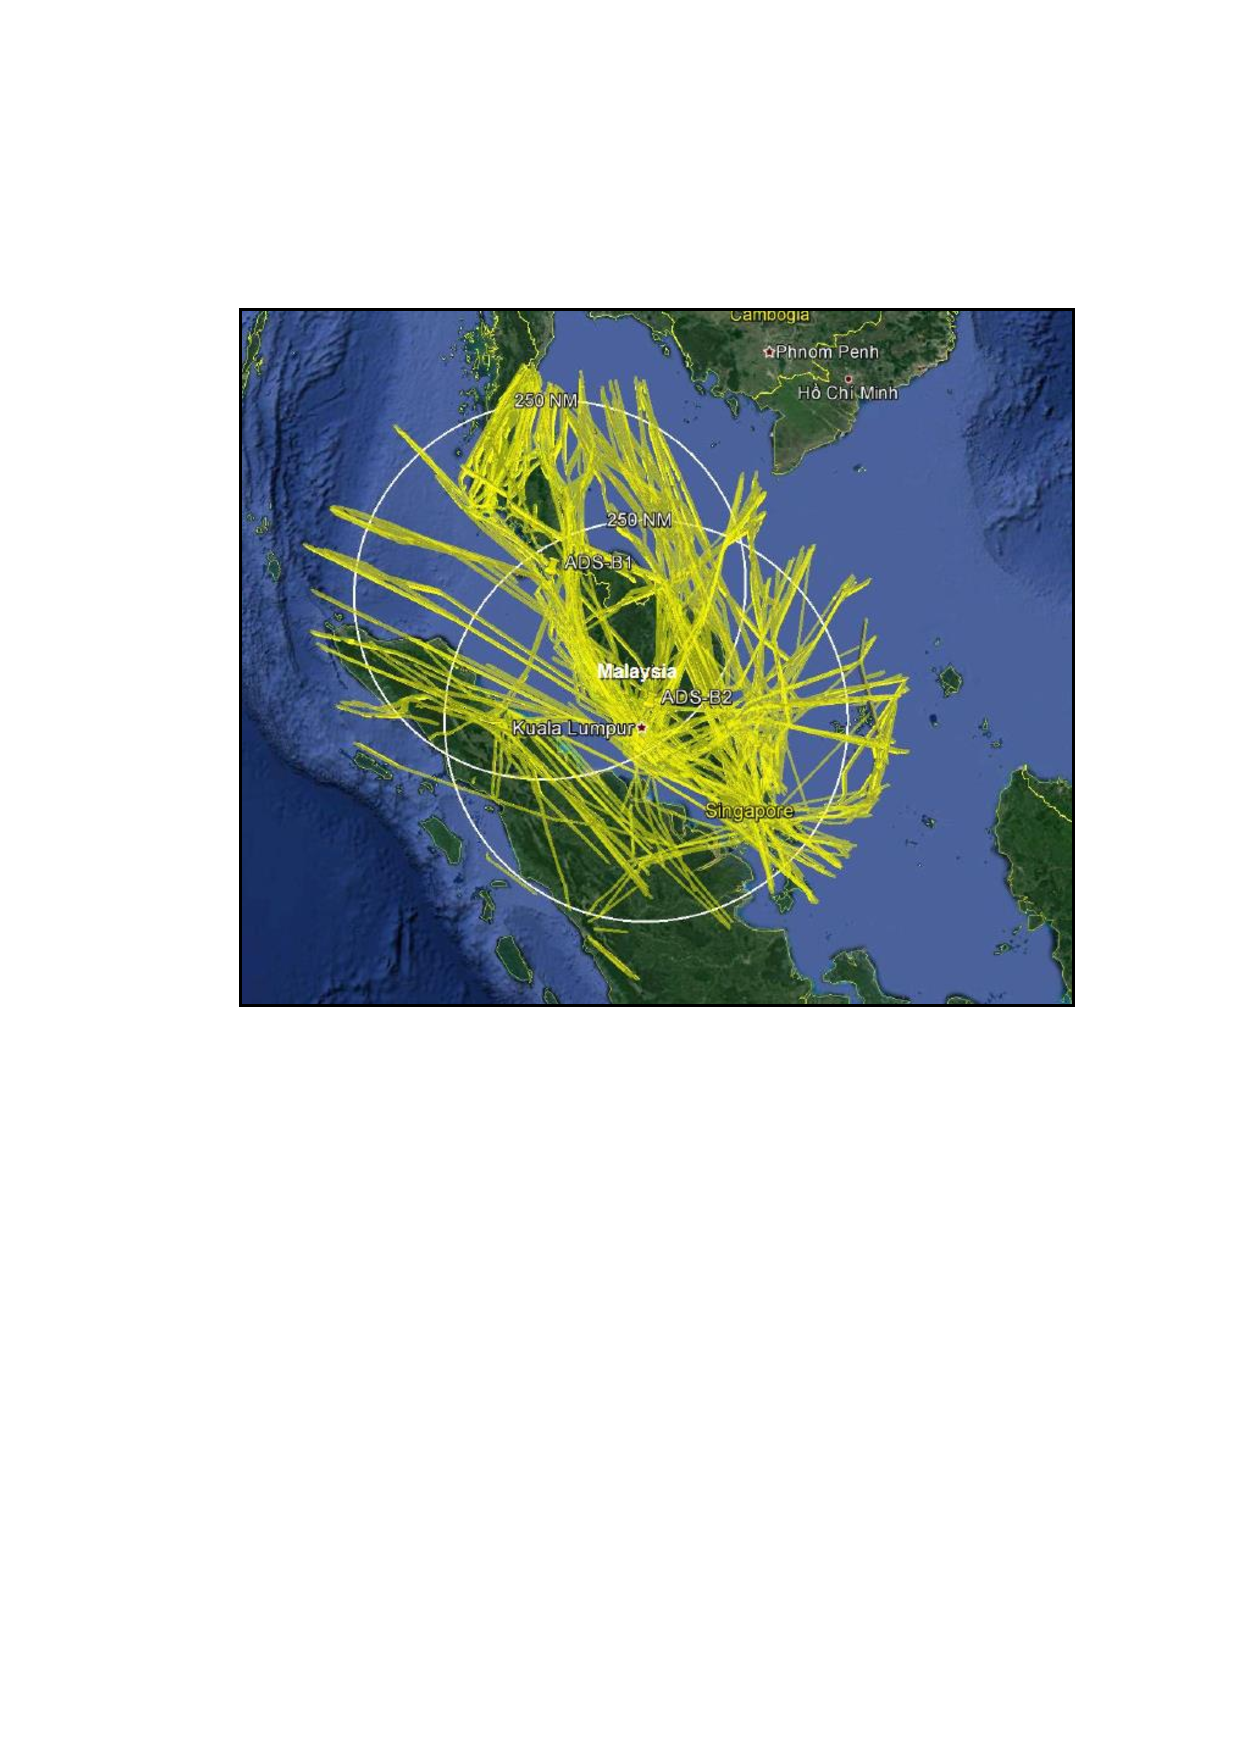
\includegraphics[width=7.5cm]{pic/Malaysia.pdf}
\caption{马来西亚航迹}
\label{fig:Malaysia}
\end{minipage}
\end{figure}

\begin{figure}[htbp]

\end{figure}

\subsubsection{泰国}

\begin{figure}[htbp]
\centering
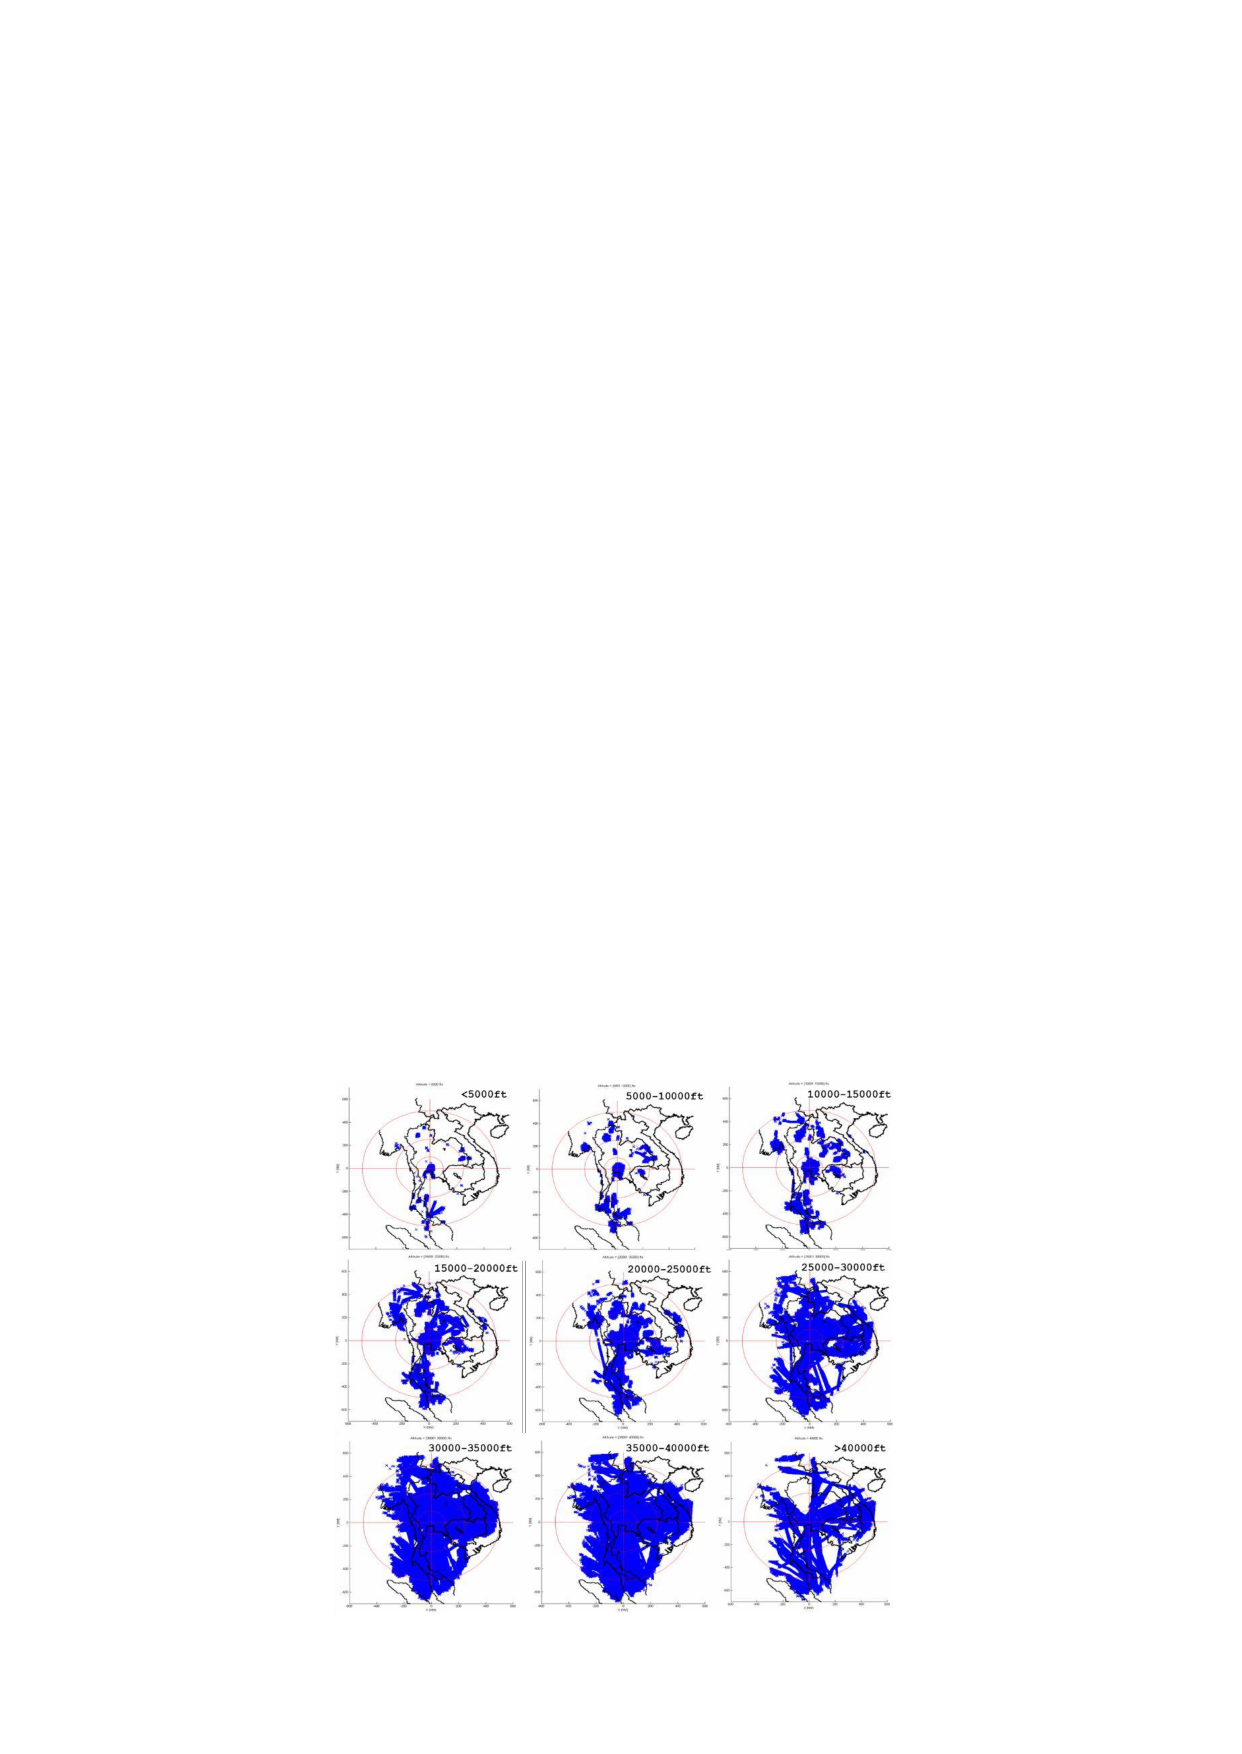
\includegraphics[width=13cm]{pic/thailand.pdf}
\caption{泰国}
\label{fig:thailand}
\end{figure}

\subsubsection{菲律宾}

\begin{figure}[htbp]
\centering
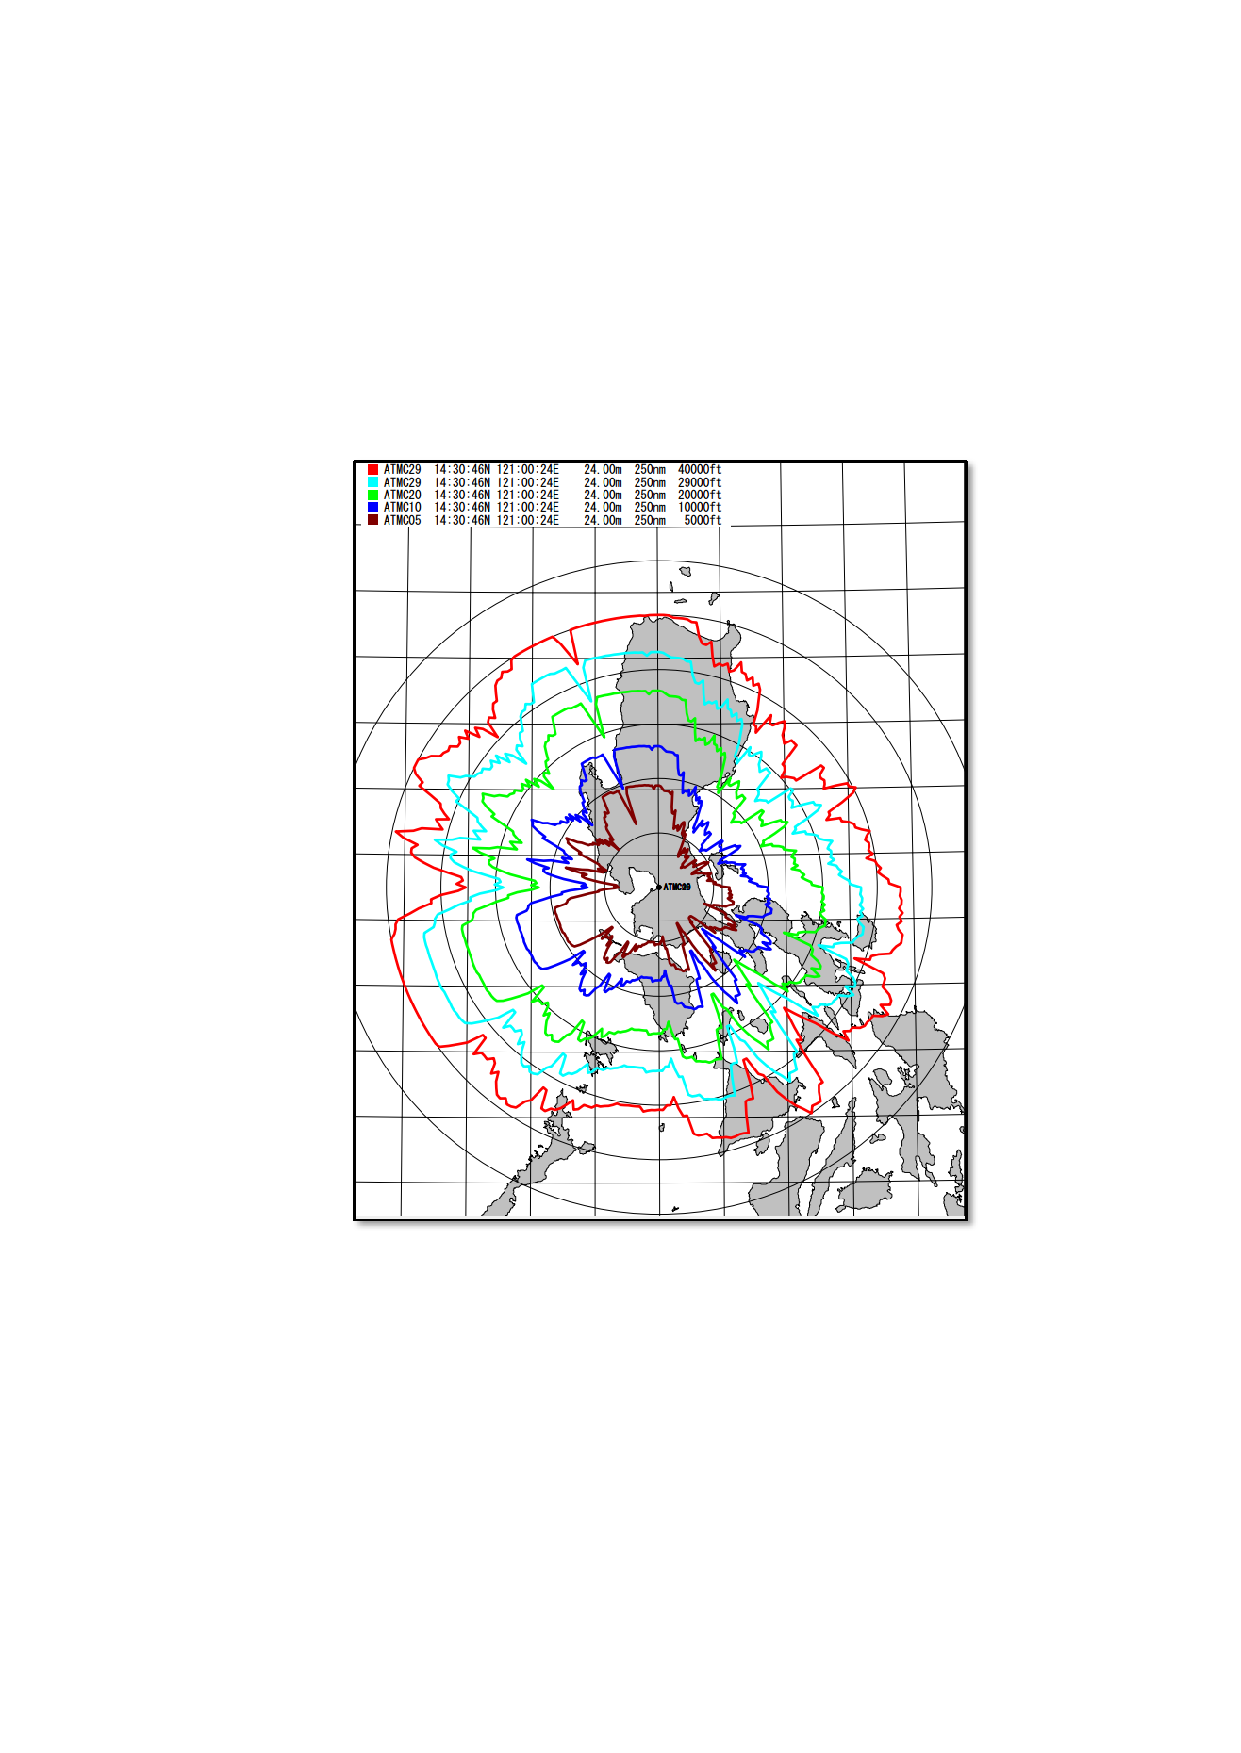
\includegraphics[width=7cm]{pic/phillipine.pdf}
\caption{菲律宾}
\label{fig:phillipine}
\end{figure}



